\chapter{Interacción CME-CME: Fenómeno}

\begin{flushright}
\begin{minipage}{0.6\textwidth}
\raggedleft 
\footnotesize\itshape
\setlength{\baselineskip}{12pt} 
\vspace{0.7cm} 
''Entonces la tormenta estalló, y los dragones danzaron.''\\
\medskip
\vspace{0.3cm} 
- George R.R. Martin, \textit{Fire \& Blood}
\end{minipage}
\end{flushright}
\vspace{1cm}


Nuestra simulación busca estudiar el comportamiento de la densidad y la velocidad de las CMEs durante su interacción, incorporando una componente estocástica en la morfología de sus perfiles que reproduce la variabilidad natural observada en estas estructuras. Esto se sustenta en el carácter recurrente y estocástico de las propias CMEs como fenómeno solar, al tratarse de eventos que ocurren repetidamente con parámetros cinemáticos y morfológicos variables, existe una probabilidad no nula de que dos o más eyecciones sucesivas lleguen a interactuar en el medio interplanetario. A través de los visualizadores de los perfiles cinemáticos y los mapas de densidad y velocidad resultantes se facilita la comprensión y el estudio cualitativo de la evolución de la interacción, al tiempo que dicha aleatoriedad controlada permite un tratamiento estadístico prospectivo, mediante la generación de múltiples simulaciones bajo distintas semillas, para caracterizar la distribución de los parámetros de interacción y su sensibilidad a la morfología inicial. 

\begin{figure}[h]
    \centering
	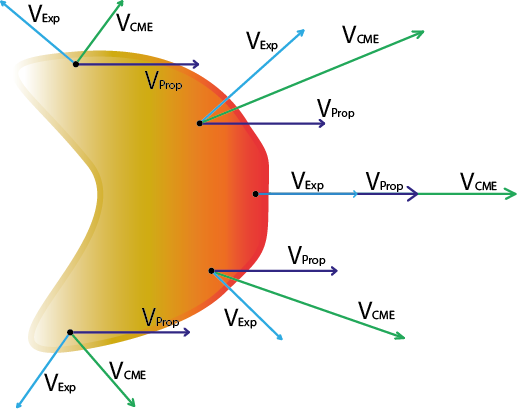
\includegraphics[width=0.65\linewidth]{imag/VectoresCME.png}
	\caption[Esquema de la superposición de las velocidades de expansión y propagación en 2D de una CME]{Representación del frente de una CME junto con la velocidad de propagación $\vec{v}_{\text{Prop}}$ (azul oscuro) y de expansión $\vec{v}_{\text{Exp}}$ (azul claro) en puntos cualquiera de la CME. El vector $\vec{v}_{\text{Exp}}$ tiene dirección radial al centro de la CME, mientras que el vector $\vec{v}_{\text{Prop}}$ tiene una dirección de propagación hacia la derecha, en todo punto de la CME. Además, el vector resultante de la superposición es $\vec{v}_{CME}$ (verde) y cambia de dirección según el punto dentro de la CME. \textit{Nota:} Figura de elaboración propia.}
    \label{CME1Boseto}
\end{figure}

Para construir el perfil de velocidad total ($\vec{v}_{\text{CME}}(r,\theta)$) de la CME precursora (CME--1), así como de la sucesora (CME--2 y 3), se debe considerar tanto su propagación (flechas en azul oscuro) como su expansión (flechas en azul claro) en coordenadas polares ($r$, $\theta$) en cada punto dentro de la CME, como lo muestra la Figura \ref{CME1Boseto}. Por lo que, $\vec{v}_{\text{Exp}}$ está en dirección radial hacia afuera del centro de la CME, mientras que el vector $\vec{v}_{\text{Prop}}$ apunta hacia la derecha, radial al Sol (fuera de la imagen, a la izquierda). Además, el vector resultante de la superposición del vector propagación y expansión, se muestra como $\vec{v}_{CME}$ (flechas en verde) y cambia de dirección según la velocidad de propagación y de expansión, de la forma
\begin{equation*}
\vec{v}_{\text{CME}}(r,\theta)=\vec{v}_{\text{Prop}}(r,\theta)+\vec{v}_{\text{Exp}}(r,\theta).
\end{equation*}
Esta dependencia angular explícita facilita el control de perturbaciones anisotrópicas, acercando la simulación a un caso más realista de CME. De manera similar, la aceleración total ($\vec{a}_{\text{CME}}(r,\theta)$) se toma como la suma de la aceleración de propagación ($\vec{a}_{\text{Prop}}(r,\theta)$) y de expansión ($\vec{a}_{\text{Exp}}(r,\theta)$), de la forma
\begin{equation*}
\vec{a}_{\text{CME}}(r,\theta)=\vec{a}_{\text{Prop}}(r,\theta)+\vec{a}_{\text{Exp}}(r,\theta).
\end{equation*}

En una segunda etapa se busca simular una CME sucesora (CME--2 y 3), de la misma manera en la que se hizo para la CME--1, pero buscando una velocidad de propagación relativamente mayor que permita una interacción con la CME precursora. Por lo que, para encontrar los parámetros que permitan la interacción, se desarrolla un código en lenguaje de programación Python que resuelve la cinemática de propagación en una dimensión (1D) de las CMEs al integrar la aceleración de la Ecuación \eqref{ecuaceleración},
\begin{equation*}
a(t)=\left[ \frac{1}{a_r\exp(\frac{t}{\tau_r})}+\frac{1}{a_d\exp(\frac{-t}{\tau_d})}\right]^{-1},
\end{equation*}
calculando la velocidad instantánea y posición del centro de la CME. Posteriormente, se determina el punto de intersección de las curvas de sus perfiles de posición y se interpreta como una interacción. Por consiguiente, es posible determinar umbrales de valores de los parámetros de la aceleración bajo los cuales la interacción es favorable. Sin embargo, debido a la multiplicidad de posibles variables experimentales es necesario establecer algunas como constantes, por lo que los parámetros de la CME--1 ($\tau_r$, $\tau_d$, $a_r$, $a_d$, $v_0$, $x_0$) se fijan, así como algunos parámetros de la CME--2 y 3 ($\tau_r$, $a_r$, $v_0$, $x_0$) y el tiempo de retraso entre CMEs, los cuales se seleccionan según estudios estadísticos de CMEs observadas \parencite[e.g.,][]{aschwanden-2019, ravishankar-2020}. Dado que la cinemática de la \ac{CME} precursora y el tiempo de retraso permanecerán constantes, la velocidad requerida por la sucesora para alcanzarla no variará, por lo que se espera que para lograr velocidades similares, $a_d$ sea inversamente proporcional a $\tau_d$.

La metodología diferencia dos casos de interacción, ver \autoref{Casosdeinteracción}, en los cuales se busca determinar los umbrales de los parámetros $\tau_d$ y $a_d$ de la CME--2 (Caso 1, $V_{\text{CME--1}} \ll V_{\text{CME--2}}$) y de la CME--3 (Caso 2, $V_{\text{CME--1}} < V_{\text{CME--3}}$) que favorecen la interacción, variando sistemáticamente sus valores hasta lograr el cruce entre las curvas de posición de ambas CMEs. La simulación parte de definir los parámetros que caracterizan la aceleración de las CMEs: $a_r$, $a_d$, $\tau_r$ y $\tau_d$, así como su velocidad inicial ($v_0$) y posición inicial ($x_0$). En seguida, se define la velocidad de las CMEs como la integral temporal de su aceleración correspondiente (ver Ecuación \eqref{ecuaceleración}), de igual manera la posición se define como la integral temporal de la velocidad. La Figura \ref{ejemplosimulación} muestra la interfaz del código desarrollado para visualizar simultáneamente los perfiles cinemáticos de las dos CMEs, teniendo los perfiles de aceleración, velocidad y posición ubicados de arriba hacia abajo, respectivamente; en la parte inferior se permite la manipulación de los parámetros de cada CME, así como el tiempo de retraso y de simulación, además de importar y exportar archivos de simulaciones. 

\begin{figure}[h]
    \centering
    \text{\large Interfaz del visualizador de la cinemática}
    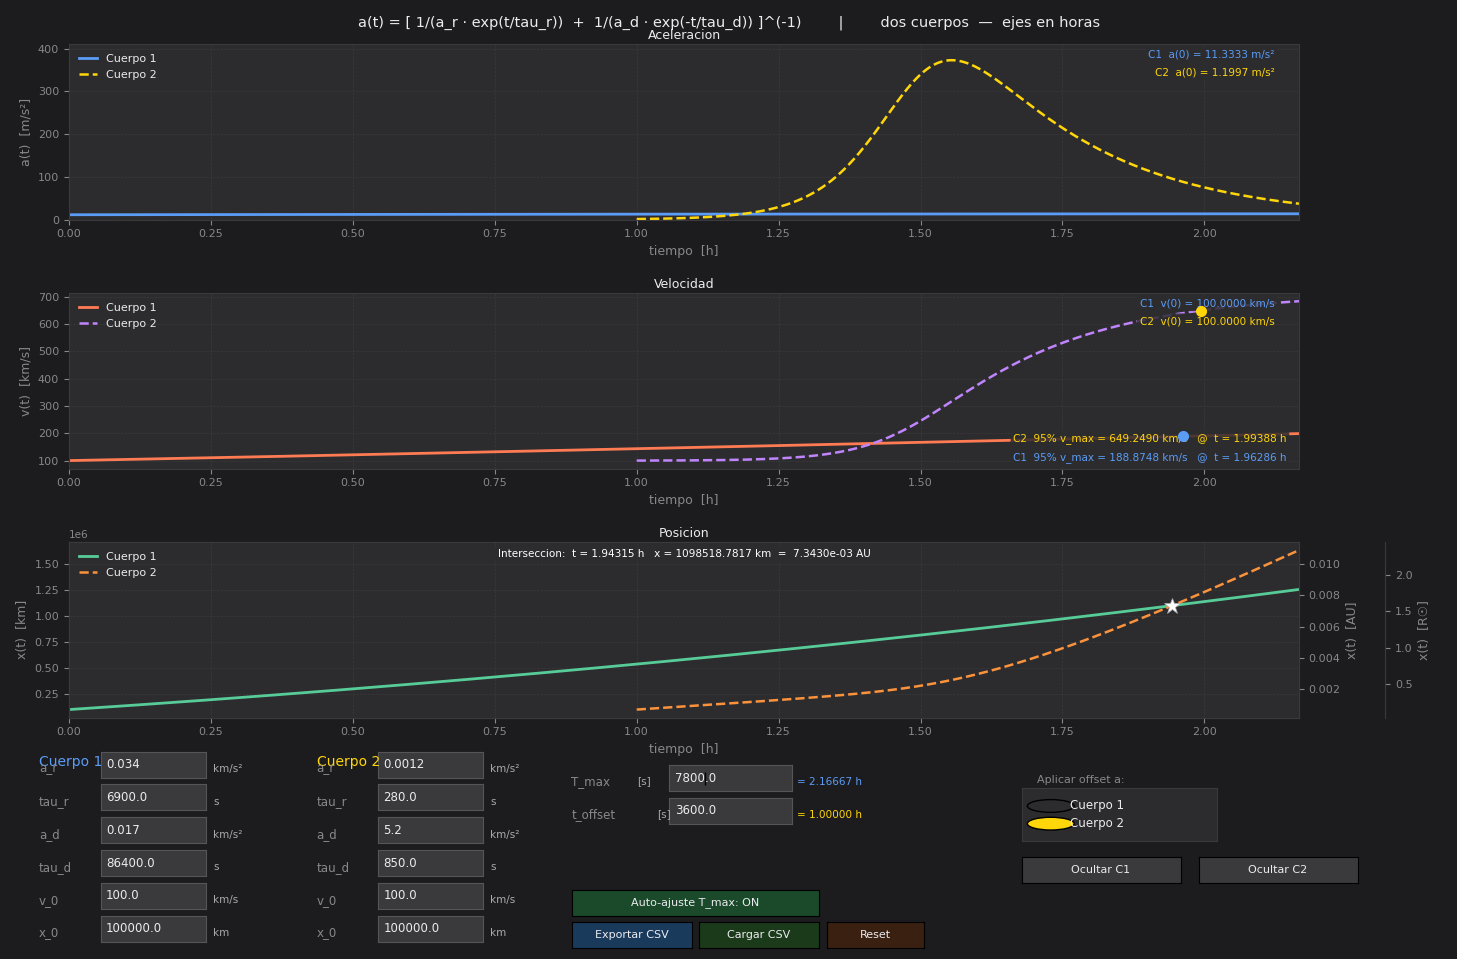
\includegraphics[width=0.9\linewidth]{imag/Ejemplo interfaz CMEs perfiles.png}
    \caption[Interfaz para visualizar perfiles cinemáticos de las CMEs]{Interfaz del programa para visualizar perfiles cinemáticos de las CMEs. Se muestra un ejemplo de CME precursora (línea sólida) y de CME sucesora (línea discontinua), así como su punto de interacción en la gráfica inferior. Los recuadros inferiores permiten la modulación de los parámetros de la aceleración, así como el tiempo de retraso y de simulación. Además se reportan aceleraciones y velocidades iniciales, además de la altura y tiempo en el que se alcanza el 95$\%$ de la velocidad máxima.}
    \label{ejemplosimulación}
\end{figure}

La propagación de las \acp{CME}\index{Coronal Mass Ejection} se representa mediante la simulación de mapas de densidad $\rho(r,\theta)$ y velocidad $v(r,\theta)$, sobre una malla polar en dos dimensiones (2D), cuya morfología es generada a partir de semillas aleatorias que alteran sus radios iniciales ($r_0$) y reproducen la variabilidad natural de las CMEs. La metodología parte de generar dos nubes de puntos randómicas que consideramos como las CMEs dentro de un \ac{SW} simulado, las cuales siguen la cinemática calculada en la simulación anterior. Las morfologías de las CMEs es alterada por aleatoriedad producida por ruido de Fourier, filamentos y asimetrías, generando una simulación mucho más realista. Por otro lado, el mapa de densidad de las CMEs tienen dos componentes: la angular y la radial, que concentran la densidad en el frente y se disipan a medida que la CME se expande.

\begin{figure}[h]
    \centering
    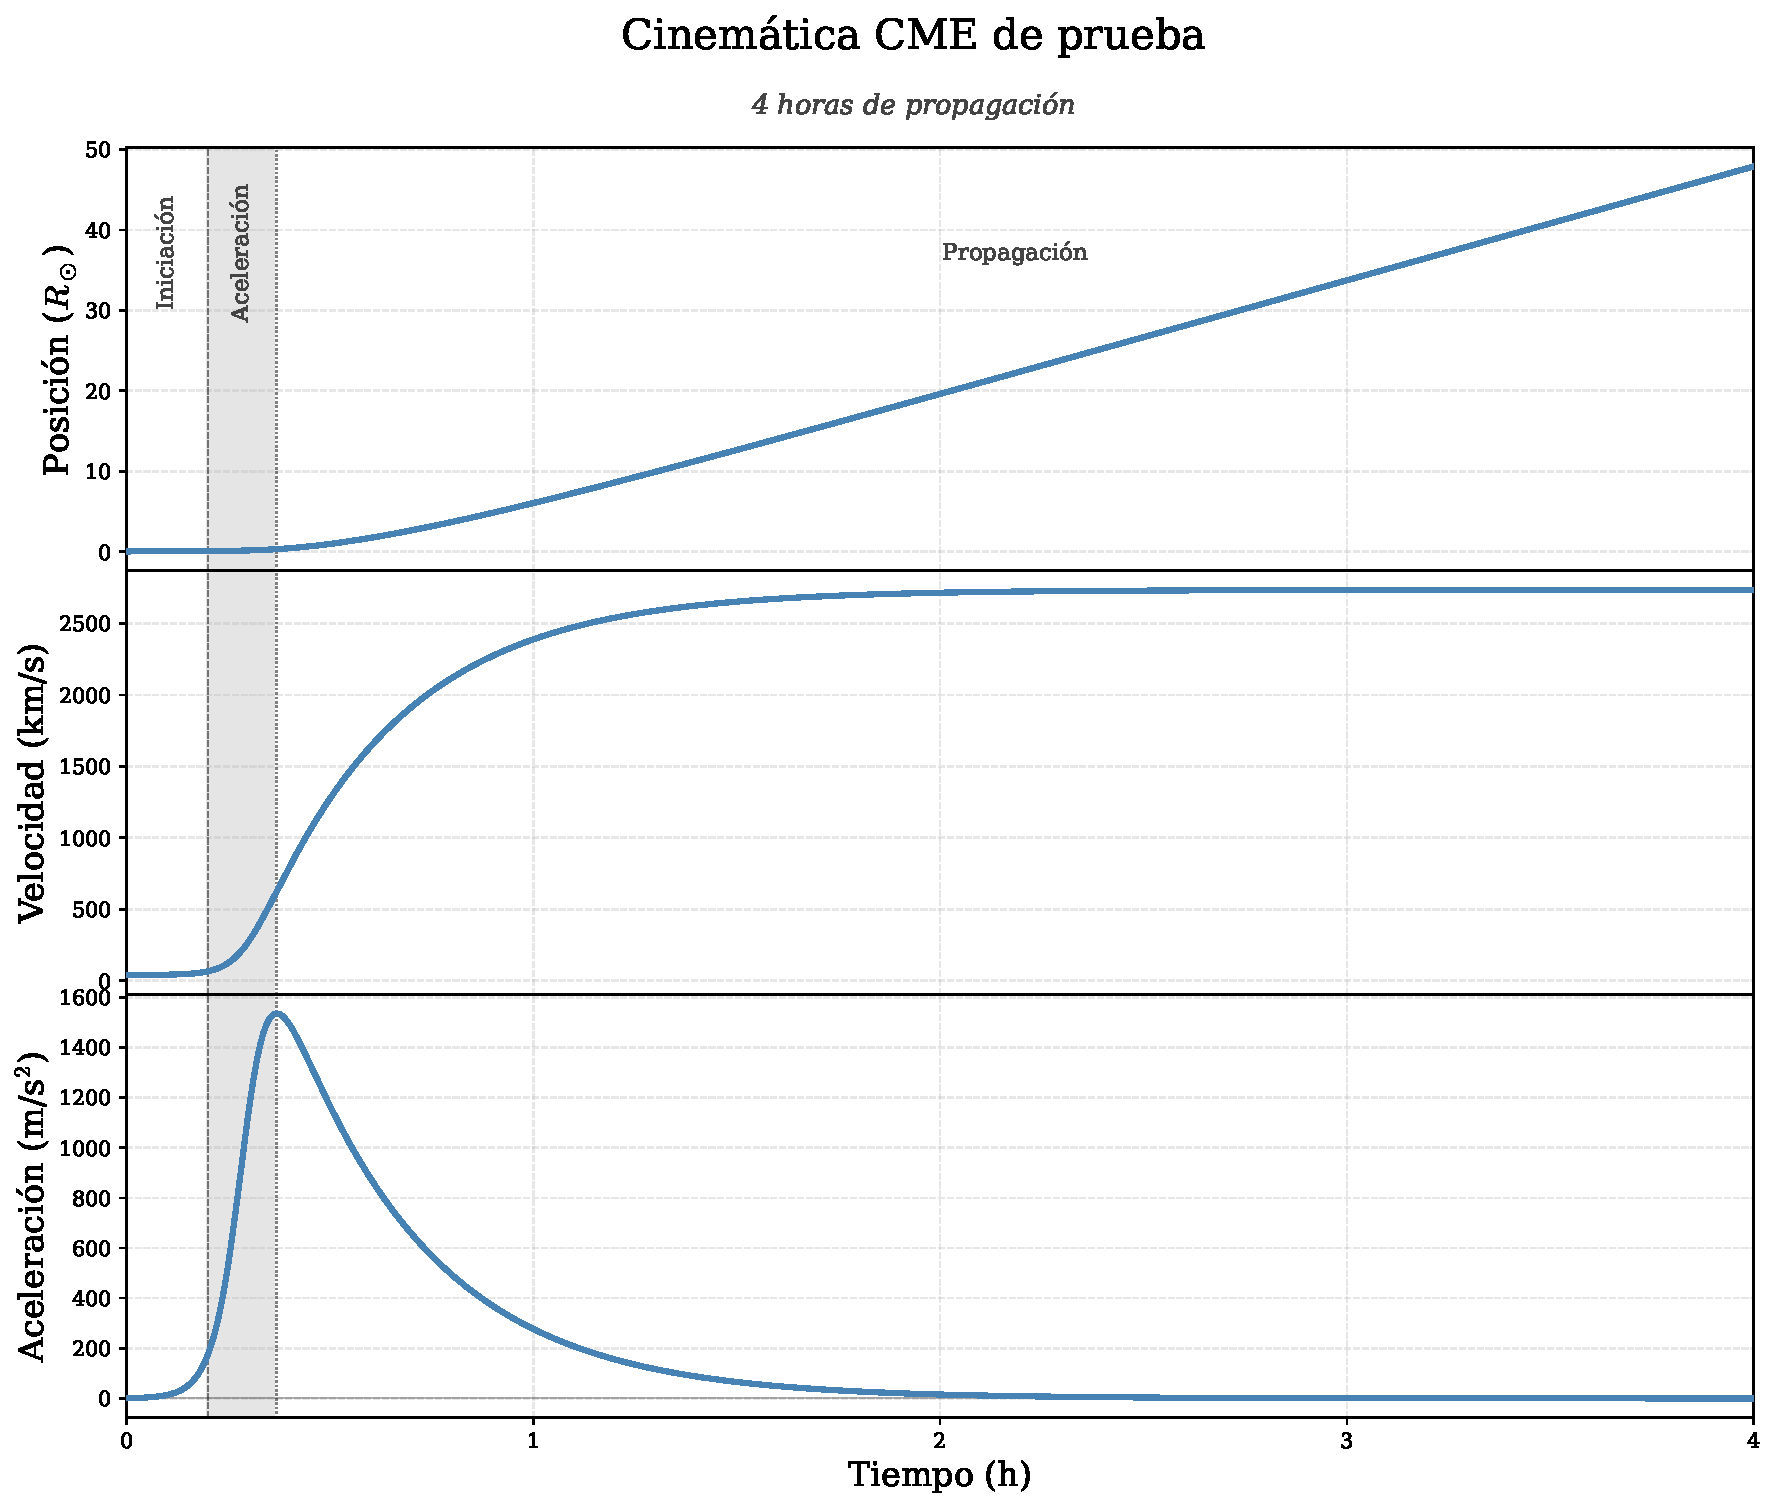
\includegraphics[width=\linewidth]{cinematica_original_prueba.pdf}
    \caption[Perfiles de posición, velocidad y aceleración para la CME de prueba]{Perfiles de posición, velocidad y aceleración para la simulación del centro de la CME reproducidos según lo reportado en \textcite[][]{gallagher-2003}\index{Gallagher}. La etapa de iniciación va desde el origen hasta la línea discontinua (blanco), la etapa de aceleración hasta la punteada (gris) y la etapa de propagación hasta el final de la gráfica (blanco); completando 10 horas de propagación en total. La línea discontinua indica el momento en el que la aceleración es máxima, mientras que la línea punteada señala el momento en el que la velocidad alcanza el $95\%$ de su velocidad máxima. \textit{Nota:} Figura de elaboración propia.}
    \label{CME1cinemática}
\end{figure}

La expansión de las CMEs toma como referencia su propagación, por lo que su frente, retaguardia y grosor se estiran o encogen en la misma proporción que crece la distancia radial desde el Sol, manteniendo siempre su forma. La forma base es un óvalo, ligeramente asimétrico, cuyos bordes se difuminan suavemente en vez de terminar de golpe. De este modo, simplemente se reescala completa a medida que avanza, conservando su morfología característica en cada instante, siguiendo lo mencionado por \textcite[][]{savani-2011} para propagaciones de CMEs en la heliosfera\index{Heliosfera} interna. Cuando entran en contacto a través de una región de solapamiento, la densidad se calcula como un promedio ponderado de las densidades individuales siguiendo la conservación de la masa, mientras que la velocidad se obtiene como un promedio ponderado por densidad, consistente con la conservación local de momento. Por lo tanto, en cada instante de la simulación surgen nuevas nubes de puntos que evolucionan de manera independiente y que, con el avance del tiempo, pueden dar lugar a nuevas regiones de interacción o de solapamiento. Adicionalmente, se generan series temporales de densidad y velocidad a distintas distancias radiales al Sol, que permiten hacer seguimiento a la evolución de la interacción en el medio interplanetario.

Para probar la fiabilidad del código, se utilizan los valores de los parámetros dados por \textcite[][]{gallagher-2003}\index{Gallagher}, los cuales reproducen los perfiles de aceleración, velocidad y posición mostrados en la Figura \ref{CME1cinemática} que coinciden con lo reportado (ver Figura \ref{fig:ejemploperfilaceleración}). La línea discontinua indica el momento en el que la aceleración alcanza el 10$\%$ de su aceleración máxima, mientras que la línea punteada señala el momento en el que la CME alcanza su máxima aceleración. Asimismo, la etapa de \textit{iniciación} se indica desde el origen hasta la línea discontinua caracterizada por bajas velocidades y aceleraciones casi nulas, la etapa de \textit{aceleración} desde la línea discontinua hasta la punteada (región gris) alcanzando velocidades de $\sim2500$ km s$^{-1}$ y aceleraciones pico de $\sim1400$ km s$^{-2}$, seguida por la etapa de \textit{propagación} desde la línea punteada hasta el final de la gráfica, donde la velocidad se estabiliza y la CME alcanza distancias de $120$ $R_\odot$ en 10 horas de simulación. El código desarrollado para esta simulación está disponible públicamente\footnote{\url{https://github.com/cristianchavez01-svg/Aproximacion-cinematica-de-la-interaccion-entre-eyecciones-de-masa-coronal-homologas.git}}, así como los códigos de las simulaciones a continuación.

\section{Resultados de interacción: Caso 1}
\label{ResultadosCaso1}
Para el Caso 1 se utiliza la CME precursora \textit{CME--1}, la cual representa una población con velocidades moderadas ($\sim600$ km s$^{-1}$), además de la CME sucesora \textit{CME--2}, que se caracteriza por tener una etapa de aceleración pronunciada e intensa durante un intervalo de tiempo corto con respecto a la CME--1, lo que conlleva a una rápida aceleración. Los detalles de sus parámetros cinemáticos, así como los resultados encontrados, se discuten a continuación.

\subsection{Cálculo de perfiles cinemáticos}

La cinemática seleccionada para la CME--1 utiliza los parámetros $\tau_r=6900$ s, $\tau_d=55600$ s, $a_r=0.034$ km s$^{-2}$, $a_d=0.01$ km s$^{-2}$, $v_0=100$ km s$^{-1}$ y $x_0=100$ Mm, tomados según \textcite[e.g.,][]{aschwanden-2019, ravishankar-2020}. De las misma forma, para la CME--2 los parámetros fijos se toman como $\tau_r=3500$ s, $a_r=0.03$ km s$^{-2}$, $v_0=140$ km s$^{-1}$ y $x_0=140$ Mm, recordando que $\tau_d$ y $a_d$ serán las variables experimentales. Asimismo, se establece un tiempo de retraso entre CMEs de 7 horas \parencite[e.g.,][]{wang-2013}. Se buscan sistemáticamente los parámetros de la CME--2 que favorezcan una interacción con la CME--1, usando el visualizador de perfiles cinemáticos, ver Figura \ref{ejemplosimulación}.

\begin{table}[h]
    \centering
    \footnotesize
    \begin{threeparttable}
        \caption[Valores mínimos de los parámetros $a_d$ y $\tau_d$ para la CME--2 bajo los cuales hay interacción]{Valores mínimos de los parámetros $a_d$ y $\tau_d$ para la CME--2 bajo los cuales hay interacción en una región $<1$ AU. La CME--1 tarda $\sim 77$ horas ($\sim 3,2$) días en llegar a 1,2 AU.}
        \label{tab:parametros_decaimiento}
        \begin{tabular}{@{}c c c c c c c c@{}}
            \toprule
            \multirow{2}{*}{\#} & $a_d$ & $\tau_d$ & $V_{\text{max}}^{95\%}$ & T int & Altura int & Tiempo $V_{\text{max}}^{95\%}$ & a$_0$ \\
             & (km/s$^2$) & (s) & (km/s) & (h) & (AU) & (h) & (m/s$^2$) \\
            \midrule
            1  & 0,01 & 57200 & 666,76 & 88,2 & 1,15  & 50,80 & 7,5\\
            2  & 0,02 & 26346,2 & 607,32 & 81,37  & 1,05  & 27,55 & 12,00\\
            3  & 0,03 & 17418,44 & 581,51  & 45,00  & 0,50  & 20,73 & 15,00\\
            4  & 0,04 & 13220,78 & 564,89  & 37,94  & 0,39  & 17,57 & 17,14\\
            5  & 0,05 & 10836,35 & 554,39 & 34,64  & 0,35  & 15,80 & 18,75\\
            6  & 0,06 & 9304,87  & 547,51 & 32,85 & 0,32  & 14,69 & 20,00\\
            7  & 0,07 & 8237,66  & 542,50 & 31,63 & 0,30  & 13,92 & 21,00\\
            8  & 0,08 & 7449,99  & 538,21 & 30,80 & 0,29  & 13,31 & 21,81\\
            9  & 0,09 & 6843,49  & 535,14 & 30,16 & 0,289 & 12,87 & 22,50\\
            10 & 0,10 & 6361,09  & 532,97 & 29,63 & 0,28  & 12,53 & 23,07\\
            11 & 0,11 & 5967,43  & 531,09 & 29,30 & 0,278  & 12,26 & 23,57\\
            12 & 0,12 & 5639,51  & 529,67 & 28,96 & 0,273 & 12,03 & 24,00\\
            13 & 0,13 & 5361,67  & 527,86 & 28,62 & 0,269 & 11,81 & 24,37\\
            14 & 0,14 & 5122,85  & 526,72 & 28,42 & 0,266 & 11,65 & 24,70\\
            15 & 0,15 & 4915,11  & 525,29 & 27,22 & 0,263 & 11,48 & 25,00\\
            16 & 0,16 & 4732,51  & 524,73 & 28,06 & 0,261 & 11,37 & 25,26\\
            17 $^{a}$ & 0,17 & 4570,57  & 523,99 & 27,89 & 0,259 & 11,26 & 25,50\\
            \bottomrule
        \end{tabular}
        \begin{tablenotes}
            \small
            \item[a] Configuración en la que el tiempo de interacción converge.
        \end{tablenotes}
    \end{threeparttable}
\end{table}

Como resultado, la CME precursora alcanza una velocidad máxima de $\sim620$ km s$^{-1}$, de la cual el 95$\%$ ($608.26$ km s$^{-1}$) se desarrolla en $\sim43$ horas, así como una aceleración inicial de $7.72$ m s$^{-2}$. Además, para la CME--2 se encuentran rangos de $\tau_d$ y $a_d$ en los cuales se desarrolla un perfil de posición y velocidad que favorecen su interacción con la CME--1. Estos valores se reportan en la Tabla \ref{tab:parametros_decaimiento} junto con su aceleración inicial (a$_0$), el valor del 95$\%$ de la velocidad máxima ($V_{\text{max}}^{95\%}$) y el tiempo en el que es alcanzada, así como la altura y tiempo de la interacción. La Figura \ref{fig:advstd} muestra la distribución de puntos de $a_d$ vs $\tau_d$, junto con su curva y ecuación de ajuste, indicando una relación inversamente proporcional con una excelente correlación ($R^{2}=0.99$), además se señalan las regiones de alta y baja probabilidad de interacción en azul y rojo, respectivamente. También, en la Figura \ref{fig:advstdvstodo} se muestran las gráficas de los parámetros de interacción anteriormente mencionados en función de los parámetros cinemáticos $a_d$ (a) y $\tau_d$ (b) de la CME--2, junto a curvas de ajuste y coeficientes de correlación, de donde se evidencia una alta correlación en la mayoría de las gráficas.

\begin{figure}[h]
    \centering
    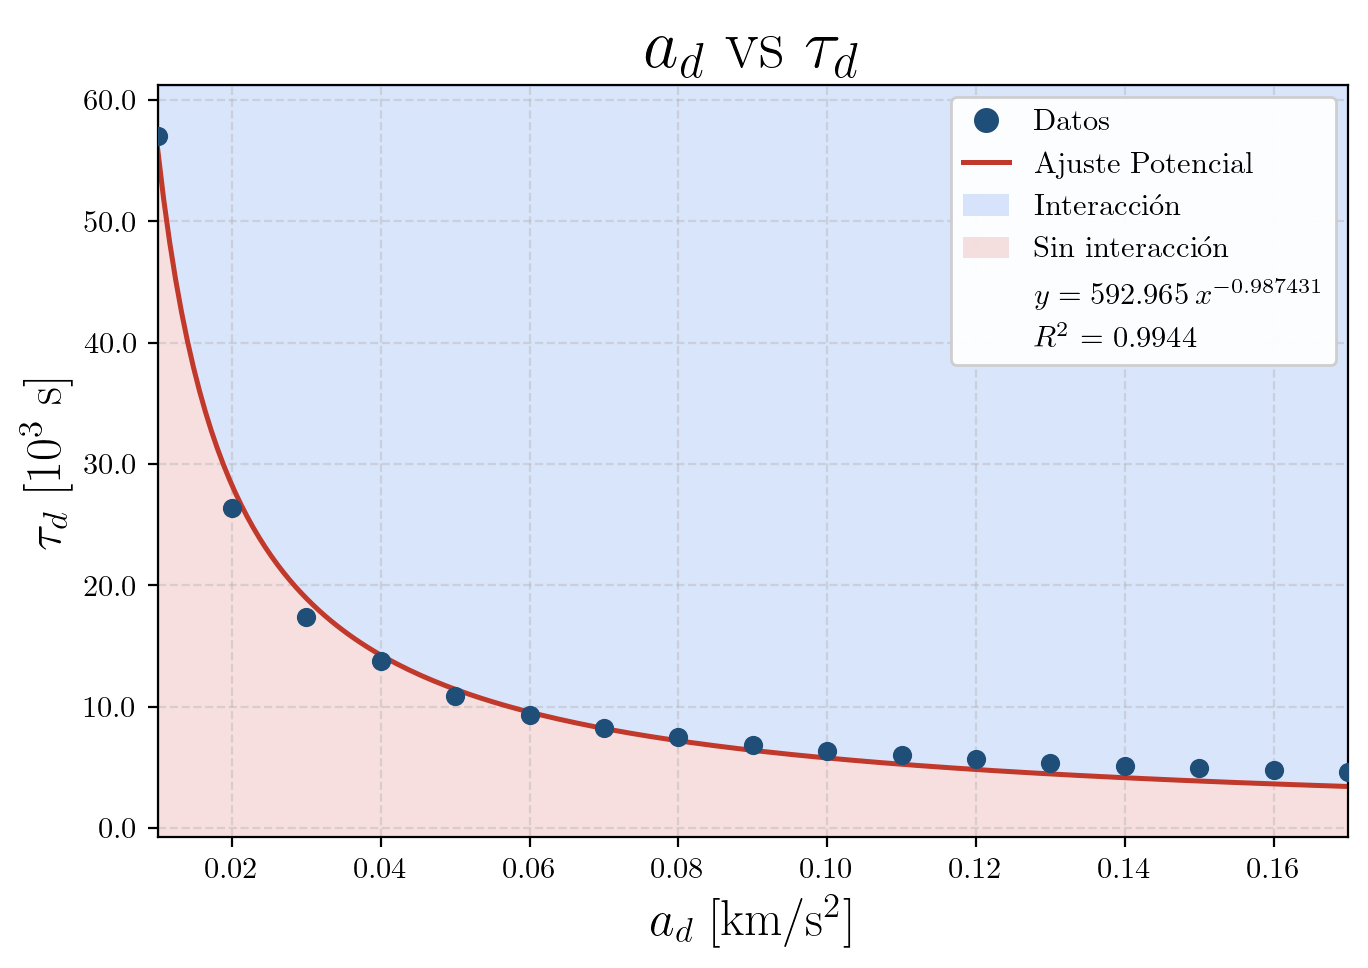
\includegraphics[width=\linewidth]{resultados/fig_ad_vs_td.png}
    \caption[Gráfica de $a_d$ vs $\tau_d$ para el Caso 1]{Gráfica de $a_d$ vs $\tau_d$, junto a la curva de ajuste (línea roja), ecuación característica y coeficiente de correlación, delimitando una región de interacción (azul) de una región en donde no la hay (roja). Los puntos en azul son los datos de la CME sucesora donde ocurre la interacción.}
    \label{fig:advstd}
\end{figure}

Para determinar las propiedades físicas de la CME resultante de la interacción se estudia en conjunto sus densidades y velocidades de las CME--1 y 2. Por lo tanto, se desarrolla el código complementario a la simulación que permite la evolución en 2D de las CMEs con mapas de densidad y velocidad en un mismo entorno, bajo los perfiles cinemáticos previamente calculados. La Figura \ref{cinematicaconjunta} muestra los perfiles de posición, velocidad y aceleración para la CME--1 (azul) y 2 (rojo) del caso $\#17$ de la Tabla \ref{tab:parametros_decaimiento}. Las regiones sombreadas en vertical delimitan las diferentes etapas en la cinemática de cada CME: iniciación (Ini) desde la producción de la CME hasta alcanzar el $60\%$ de su aceleración máxima, aceleración (Acel) desde el fin de la fase de iniciación hasta el momento en el que alcanza la aceleración máxima y propagación (Prop) de este último punto en adelante.

También, la Figura \ref{cinematicaconjunta} indica la expansión de cada CME a través de las regiones sombreadas que envuelven sus curvas de posición, siendo el frente de la CME el extremo superior de la región, el cual se encuentra más alejado del centro con respecto al borde inferior como consecuencia de la superposición de la propagación y expansión. Además, se indica (con una X) el punto de interacción de los extremos trasero y frontal de la CME precursora y sucesora, respectivamente, así como el punto de interacción entre sus centros (circulo). Por último, se indica la posición de la Tierra (línea discontinua horizontal) en el panel inferior, donde tiempo de llegada se calcula en $\sim60-65$ horas para el frente de las CMEs y $\sim80$ horas para sus centros.

\subsection{Cálculo de densidad y velocidad de la interacción}

La Figura \ref{CME1evolución} muestra la evolución de la densidad, velocidad y morfología de la CME--1 siguiendo la superposición de su propagación y expansión. El campo de velocidades es radial, centrado en el Sol, señalando tanto la expansión como la propagación de cada parte de la CME. Por otro lado, para la CME--2 se tiene el mismo módulo de código que la CME--1, produciendo una evolución mostrada en la Figura \ref{CME2evolución}, presentando una distribución de densidad y velocidad similares a la reportada para la CME--1, pero difiriendo en su morfología. 

La Figura \ref{cinematicapolarconjunta} muestra la simulación de la interacción entre las dos CMEs, en donde la densidad se indica con el mapa de color, con mínimos (morado) y máximos (amarillo). Además, el campo de velocidad (vectores rojos) señala la dirección de propagación de cada región, demostrando la superposición de una propagación y una expansión, así como la termalización de la velocidad en las regiones interactuantes en comparación a las no interactuantes. En general, la velocidad converge a valores cercanos de la velocidad de fondo. Finalmente, la interacción produce una CME resultante con una zona de mayor densidad con respecto a las CMEs individuales (ver Figuras \ref{CME1evolución} y \ref{CME2evolución}), además de un campo de velocidades homogeneizado en las zonas de interacción.

Como último resultado de la simulación, se generan series temporales de densidad y velocidad para diferentes posiciones radiales simulando la presencia de naves espaciales virtuales. La Figura \ref{Serietiempocaso1} muestra las curvas de densidad (panel superior) y velocidad (panel inferior) registradas para puntos cercanos (morado) y lejanos (rojo) al Sol, señalando incrementos durante el paso de las CMEs y su interacción; se indica el inicio de la CME-2 con una línea vertical punteada. Asimismo, en el panel de densidad se señala la densidad de fondo (10 protones cm$^{-3}$) con una línea discontinua horizontal y en el panel de velocidad se señala la velocidad del \ac{SW}\index{Solar Wind} utilizada (400 km s$^{-1}$). Nótese que al comparar las velocidades alcanzadas por las CMEs individuales ($\sim600$ km s$^{-1}$ para la CME--1 y $\sim560$ km s$^{-1}$ para la CME--2, Figura \ref{cinematicaconjunta}) y la velocidad alcanzada por la interacción ($\sim560$ km s$^{-1}$ con un pico de $\sim580$ km s$^{-1}$, Figura \ref{Serietiempocaso1}), esta última es dominada por la velocidad de la CME--2.

\begin{figure}[h]
    \centering
    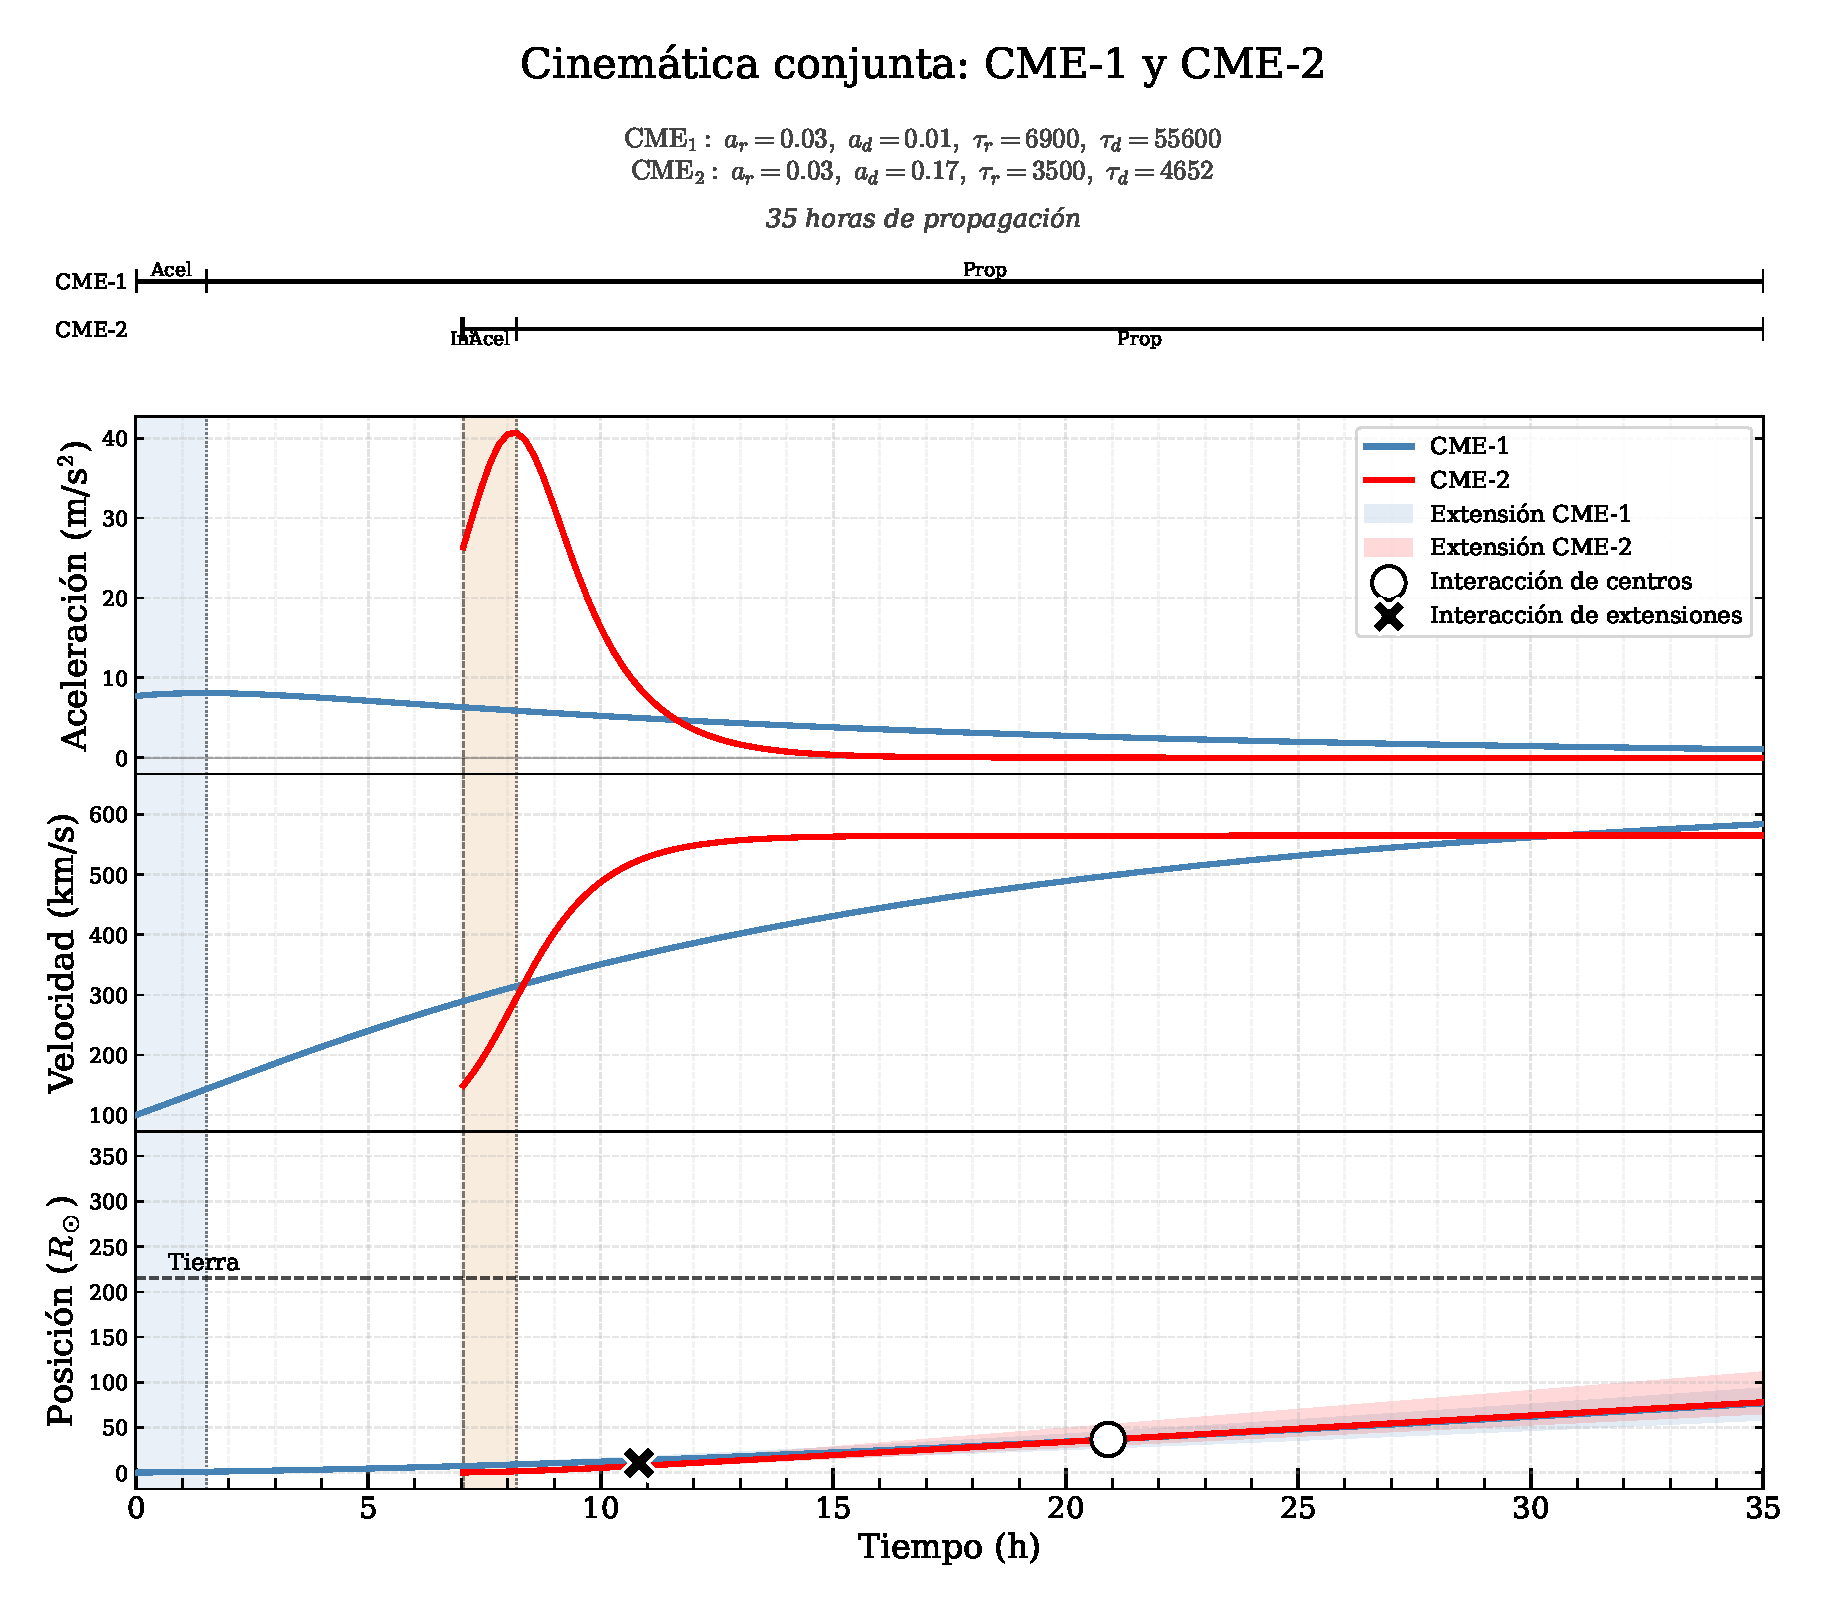
\includegraphics[width=\linewidth]{cinematica_conjunta_s1_435_s2_1962.pdf}
    \caption[Perfiles cinemáticos de las dos CMEs]{Perfiles cinemáticos de la CME--1 (azul) y CME--2 (rojo) sin presentar interacción. Además, se señalan las etapas de aceleración: iniciación (Ini), aceleración (Acel) y propagación (Prop) respectivamente para la CME--1 y 2. También, las etapas de iniciación y aceleración están separadas por una línea discontinua, mientras que las etapas de aceleración y propagación lo están con una línea punteada. La expansión de las CMEs se muestra como la región sombreada que envuelve la curva de posición de su centro. La posición de la Tierra se muestra con una línea discontinua horizontal.}
    \label{cinematicaconjunta}
\end{figure}

\begin{figure}[htbp]
    \centering
    \begin{subfigure}{\textwidth}
        \centering
        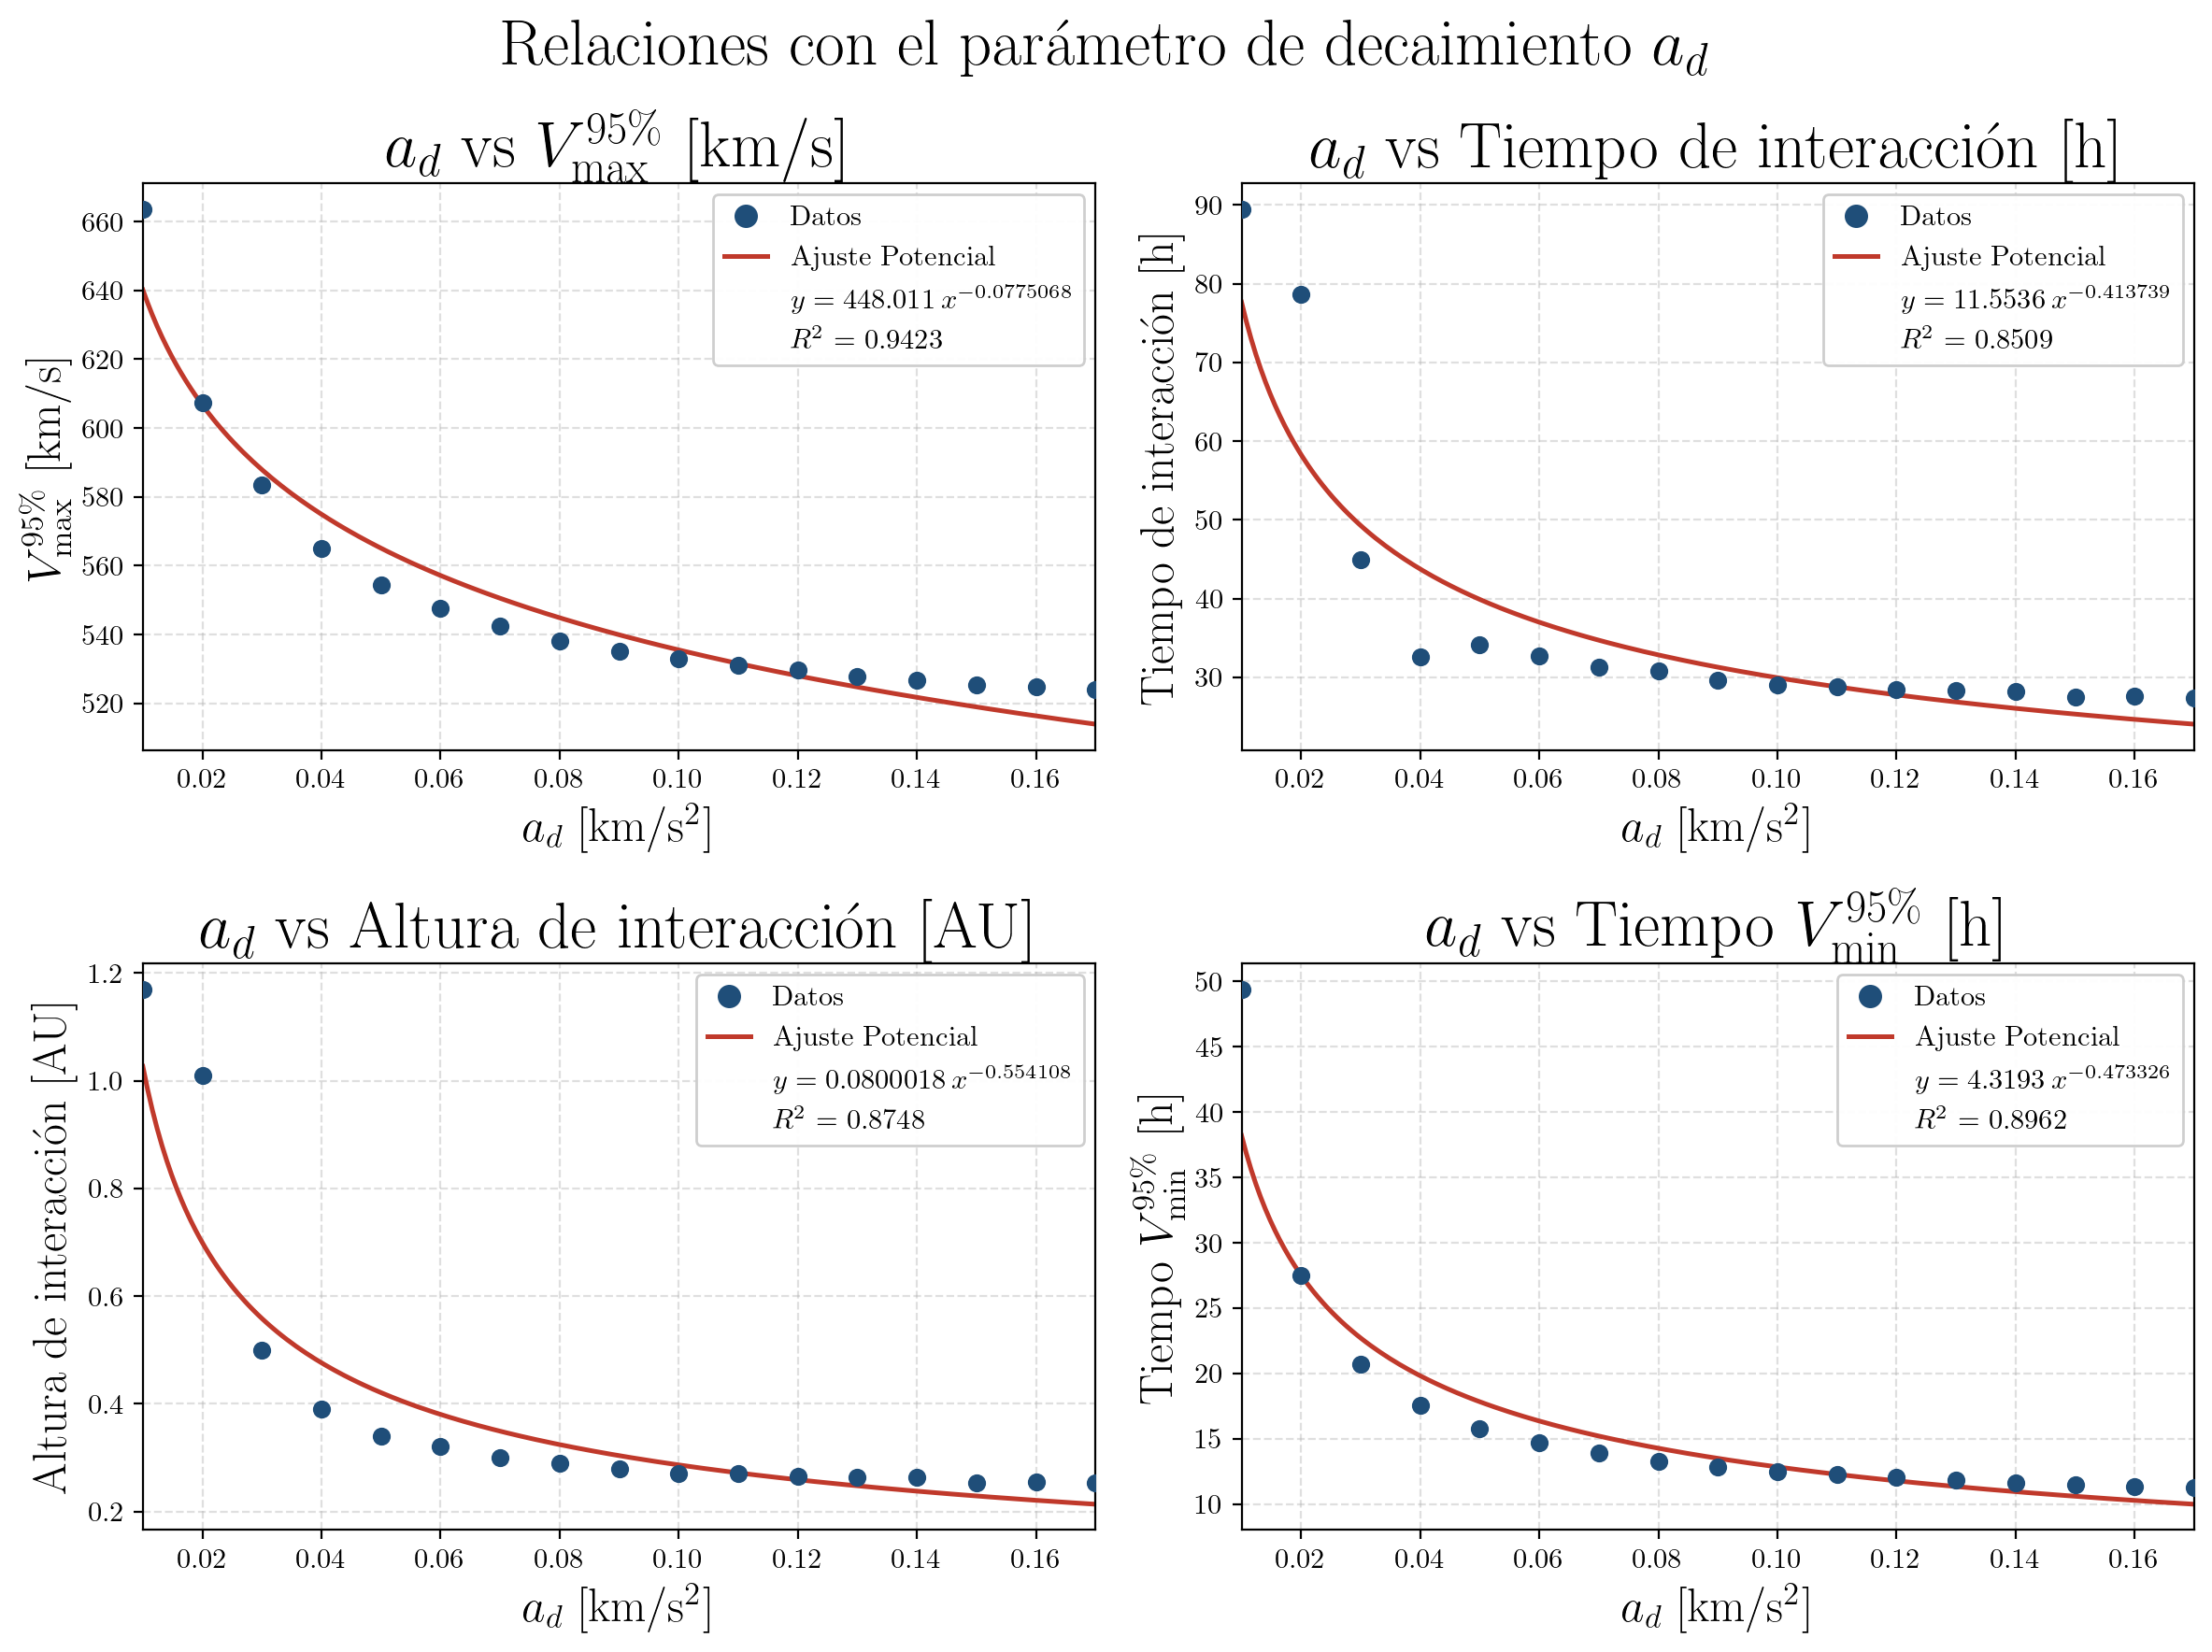
\includegraphics[width=0.9\linewidth]{resultados/fig_ad_relaciones.png}
        \caption*{(a)}
    \end{subfigure}
    \hfill
    \begin{subfigure}{\textwidth}
        \centering
        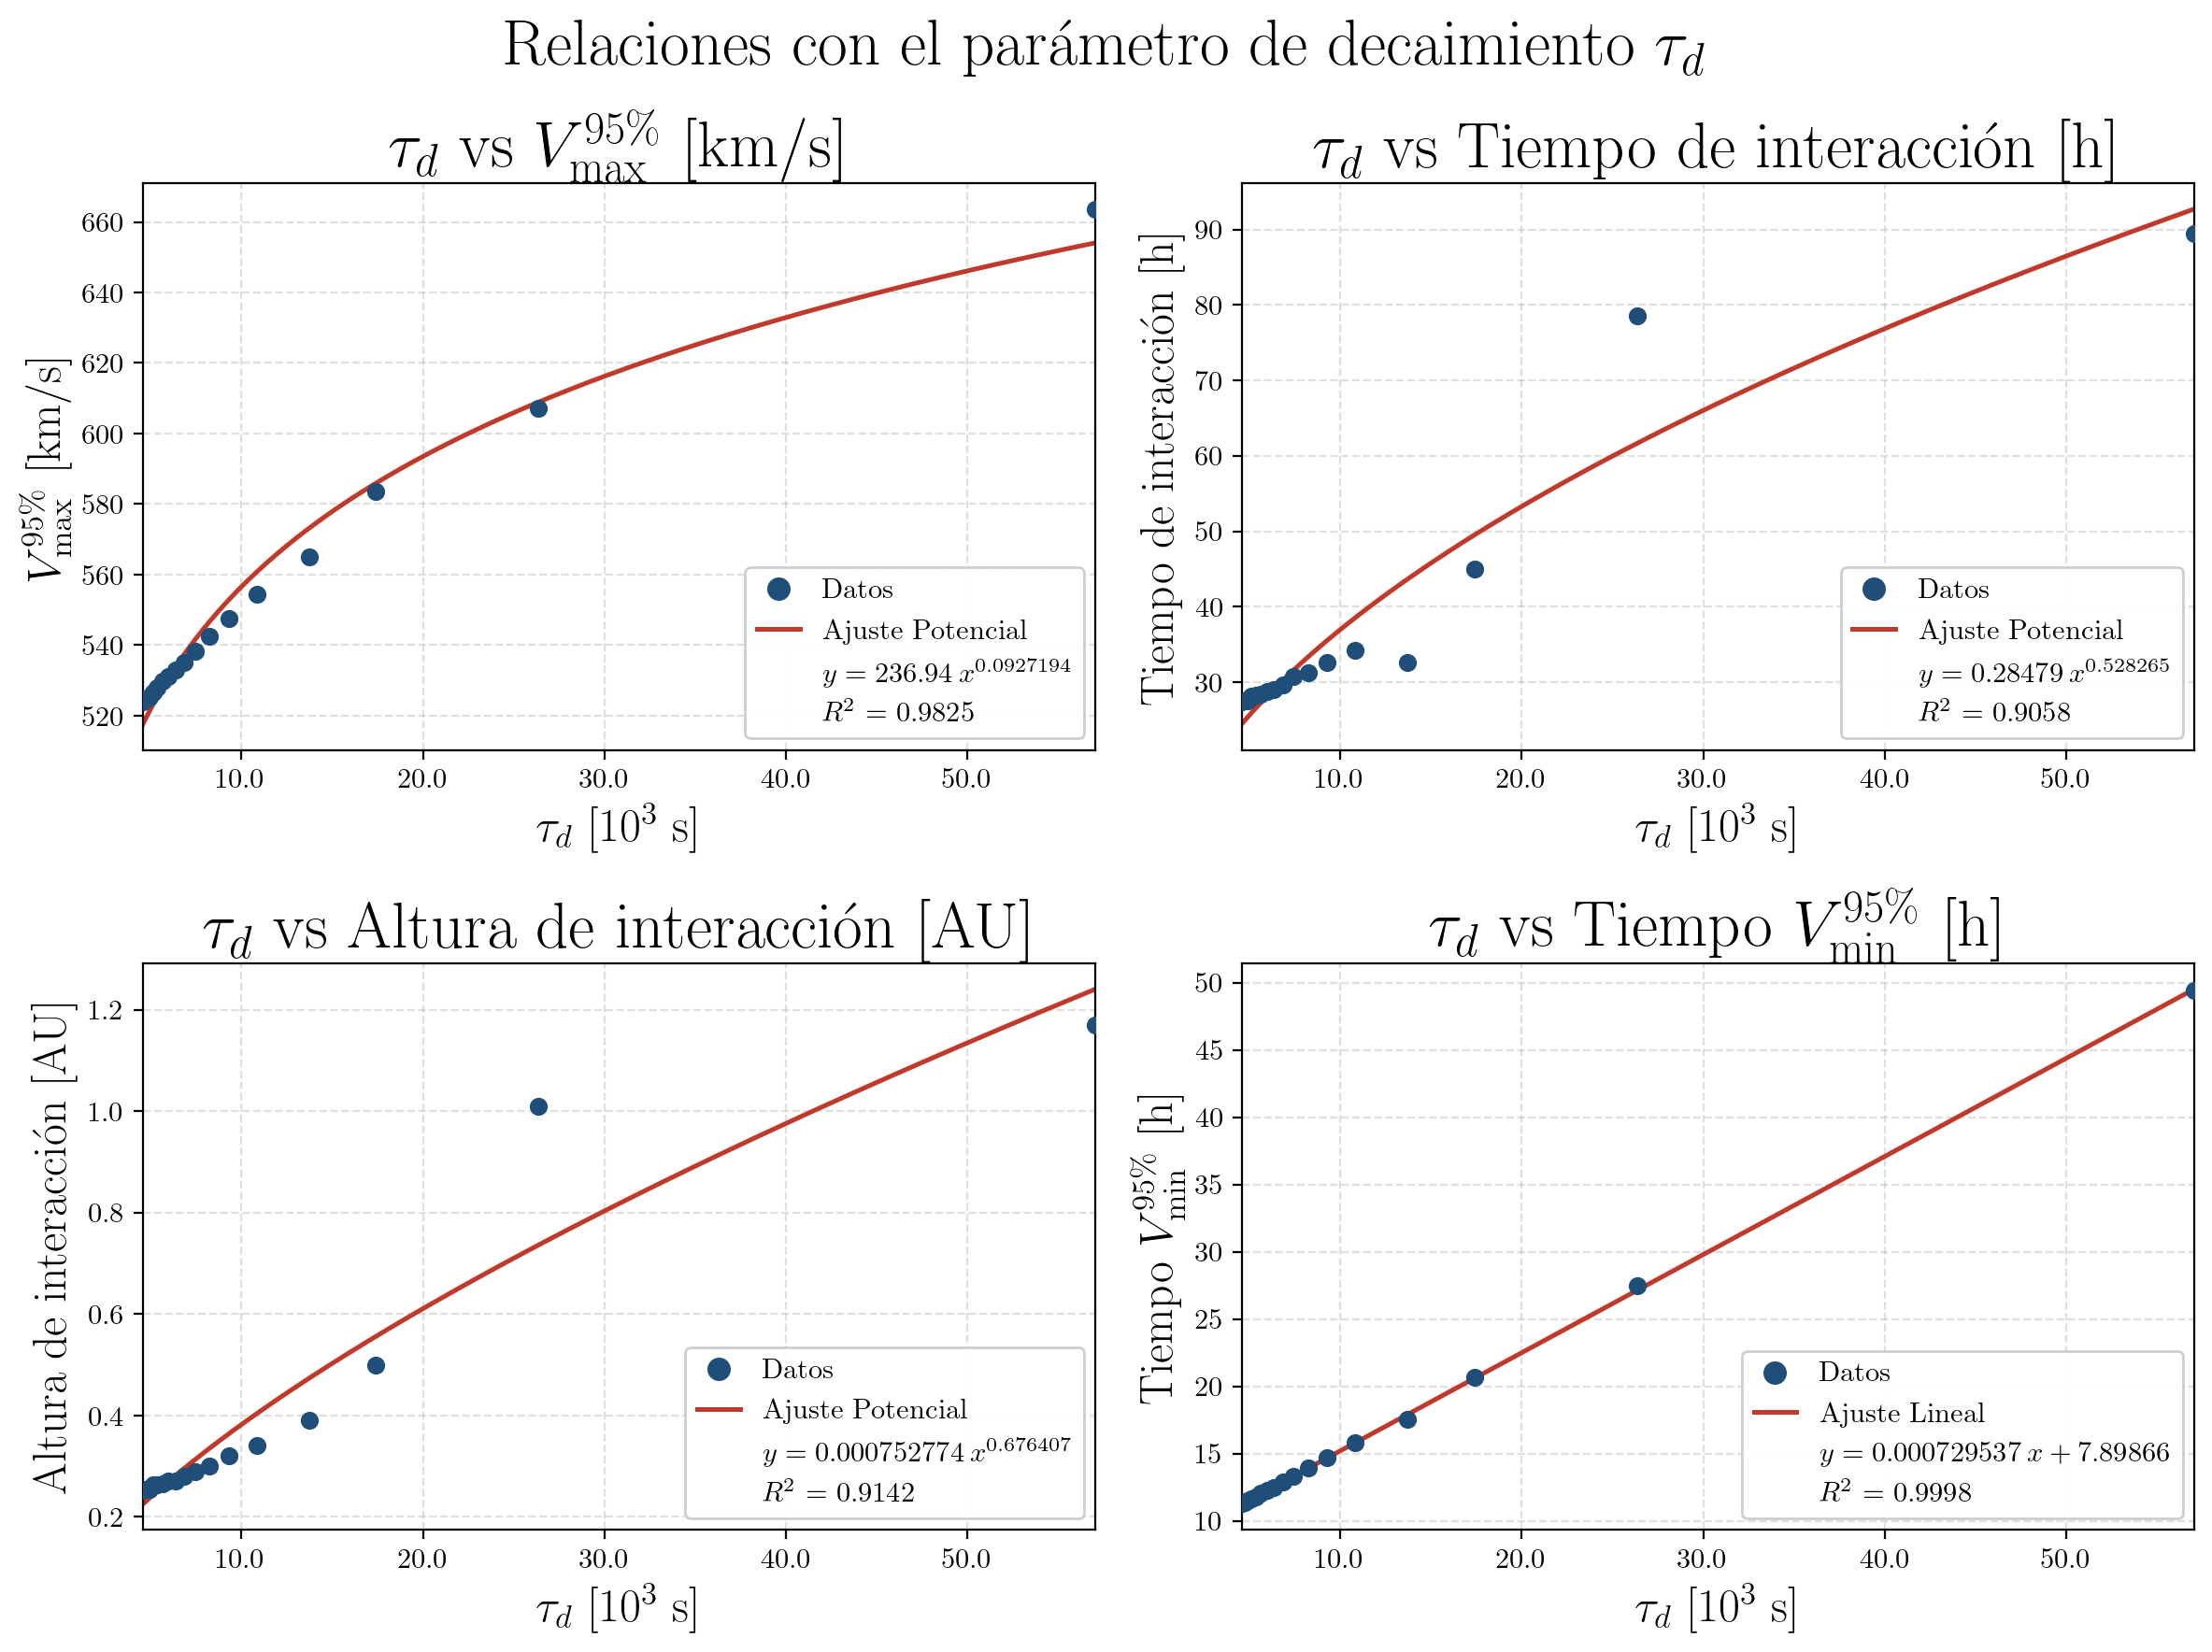
\includegraphics[width=0.9\linewidth]{resultados/fig_td_relaciones.png}
        \caption*{(b)}
    \end{subfigure}
    \caption[Gráficas de $a_d$ y $\tau_d$ vs parámetros de interacción para el Caso 1]{Gráficas de $a_d$ (a) y $\tau_d$ (b) vs parámetros de interacción para el Caso 1, junto a las curvas de ajuste (línea roja) correspondientes, ecuaciones características y coeficientes de correlación. Los puntos en azul son los datos de la CME--2 bajo los cuales ocurre la interacción.}
    \label{fig:advstdvstodo}
\end{figure}

\begin{landscape}
    \begin{figure}[p]
        \centering
        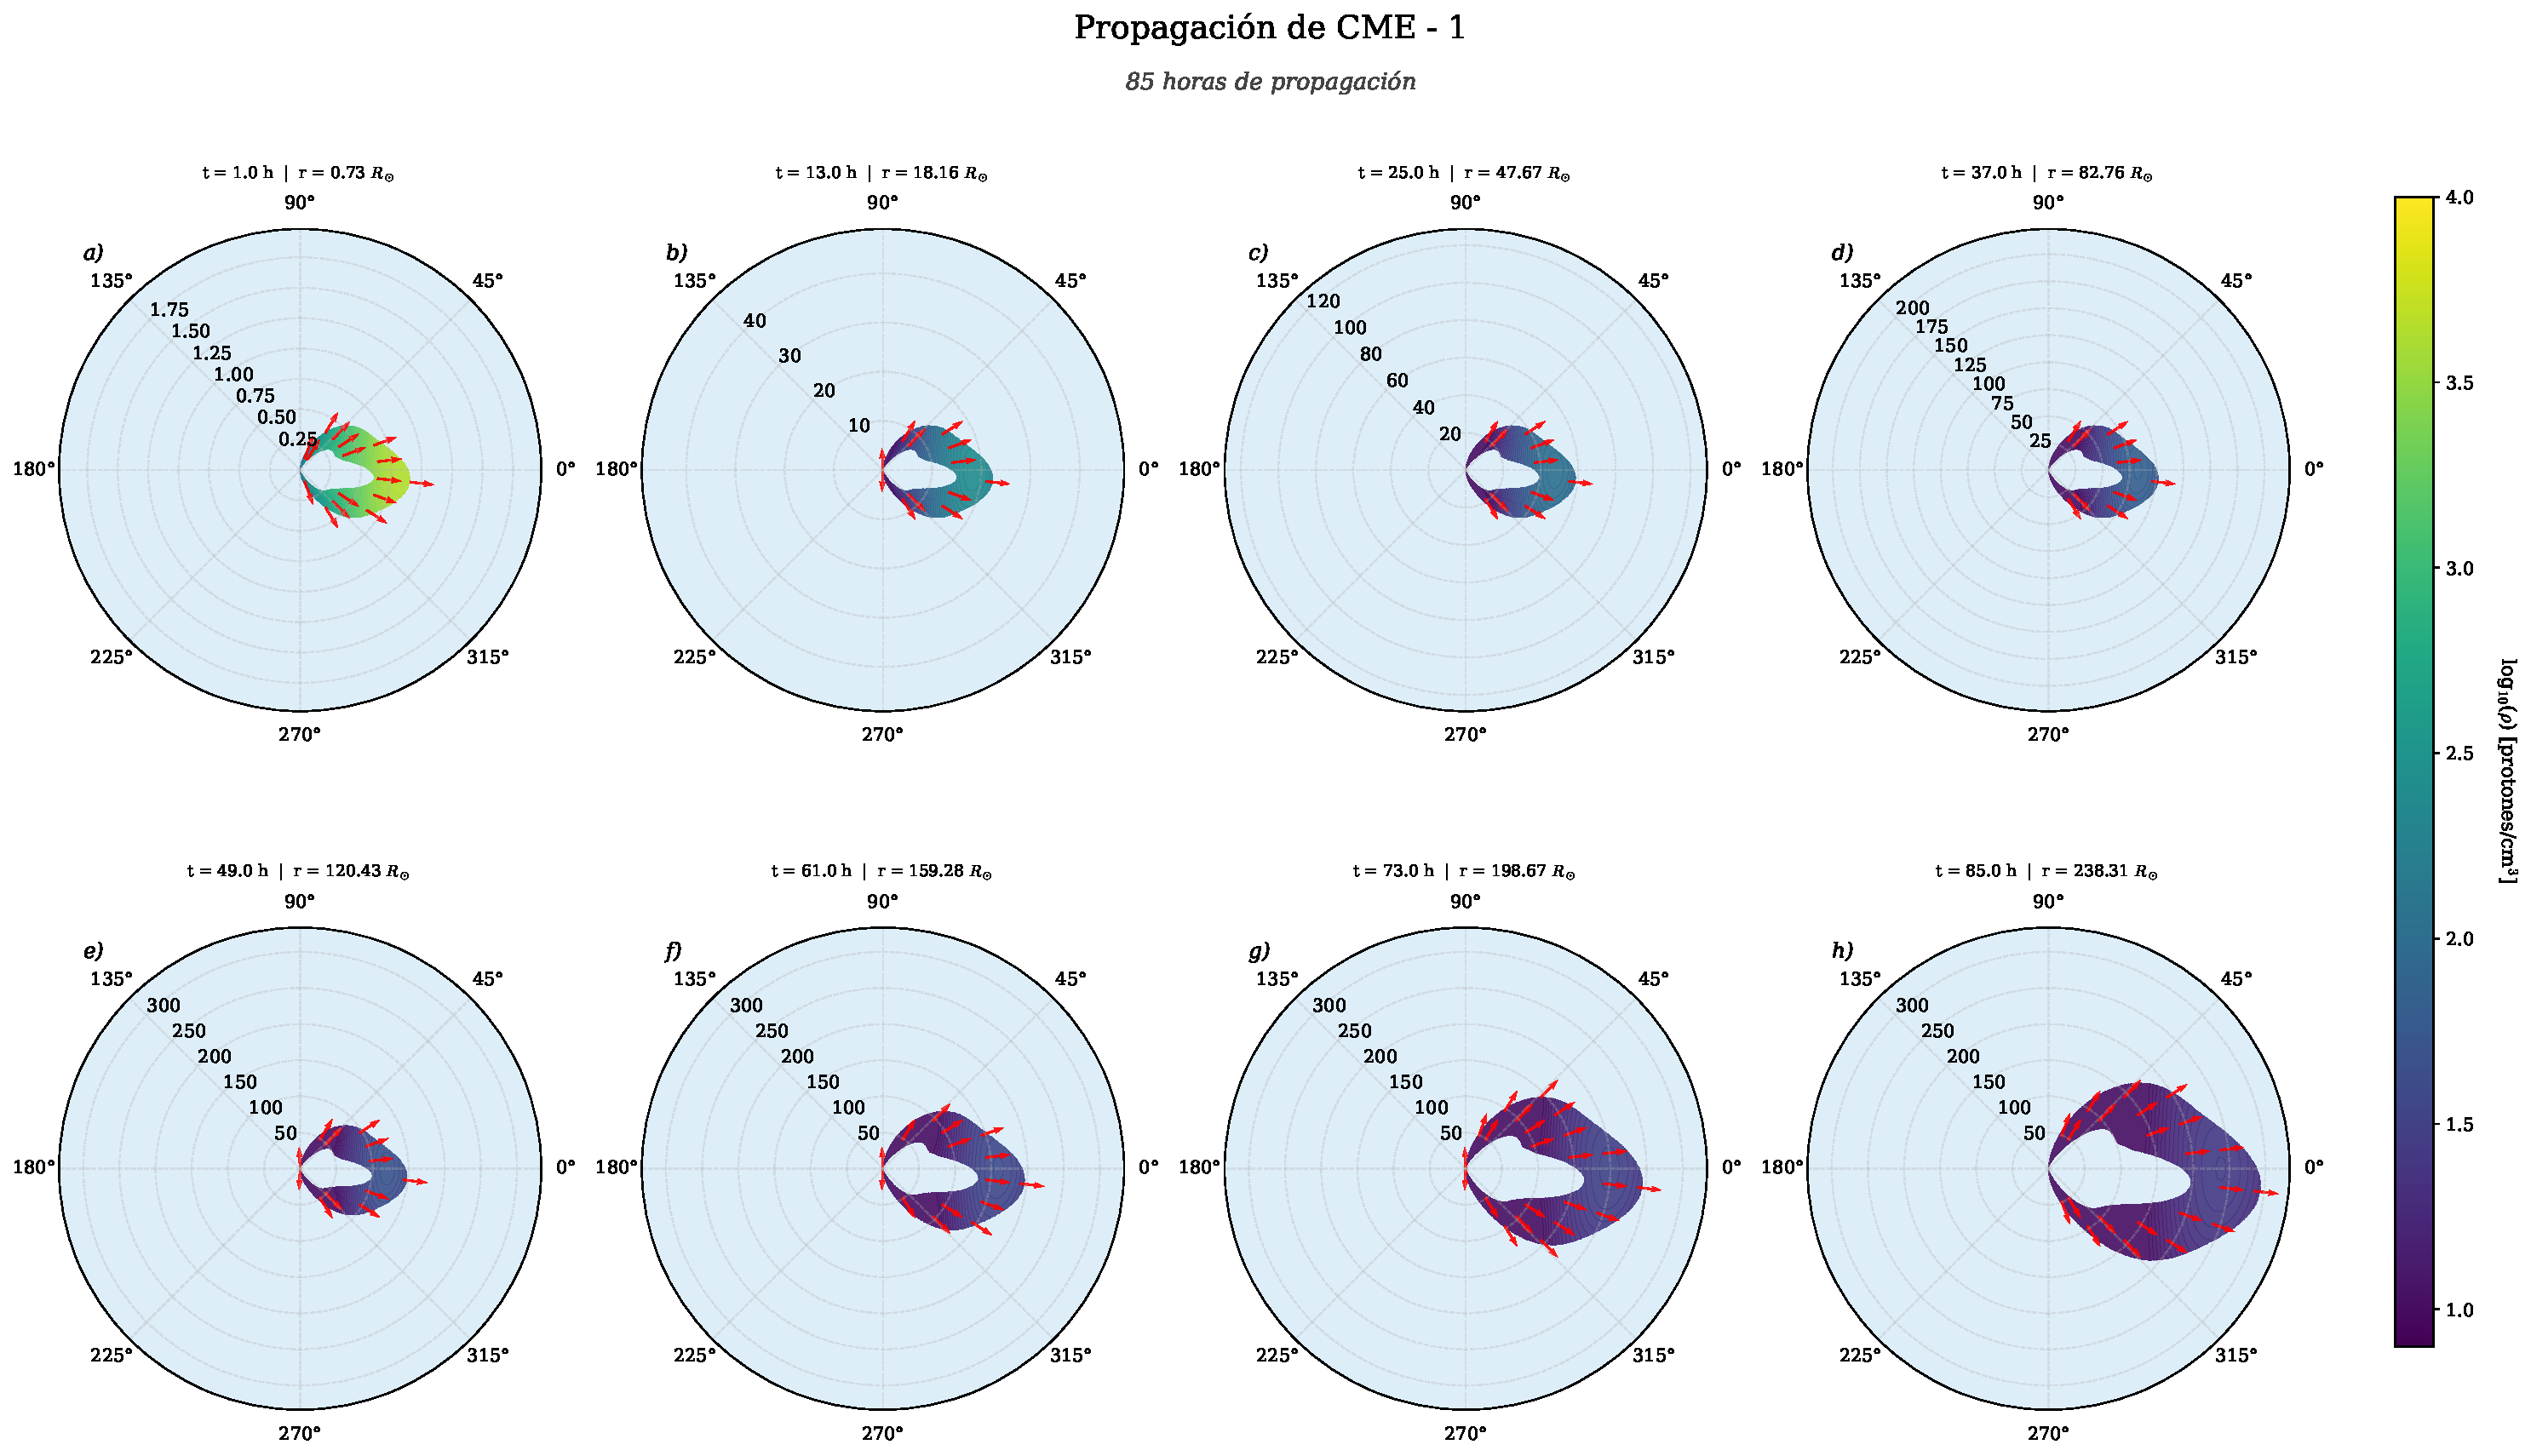
\includegraphics[width=\linewidth]{cme_evolucion_polar_precursora.pdf}
    \caption[Evolución polar de la CME precursora]{Evolución polar de la CME--1. La escala de colores representa los valores de densidad con mínimos (morado) y máximos (amarillo). La velocidad se indica a través del campo vectorial (rojo). En la parte superior de cada panel se indica el tiempo transcurrido y la posición del centro de la CME.}
    \label{CME1evolución}
    \end{figure}
\end{landscape}

\begin{landscape}
    \begin{figure}[p]
        \centering
        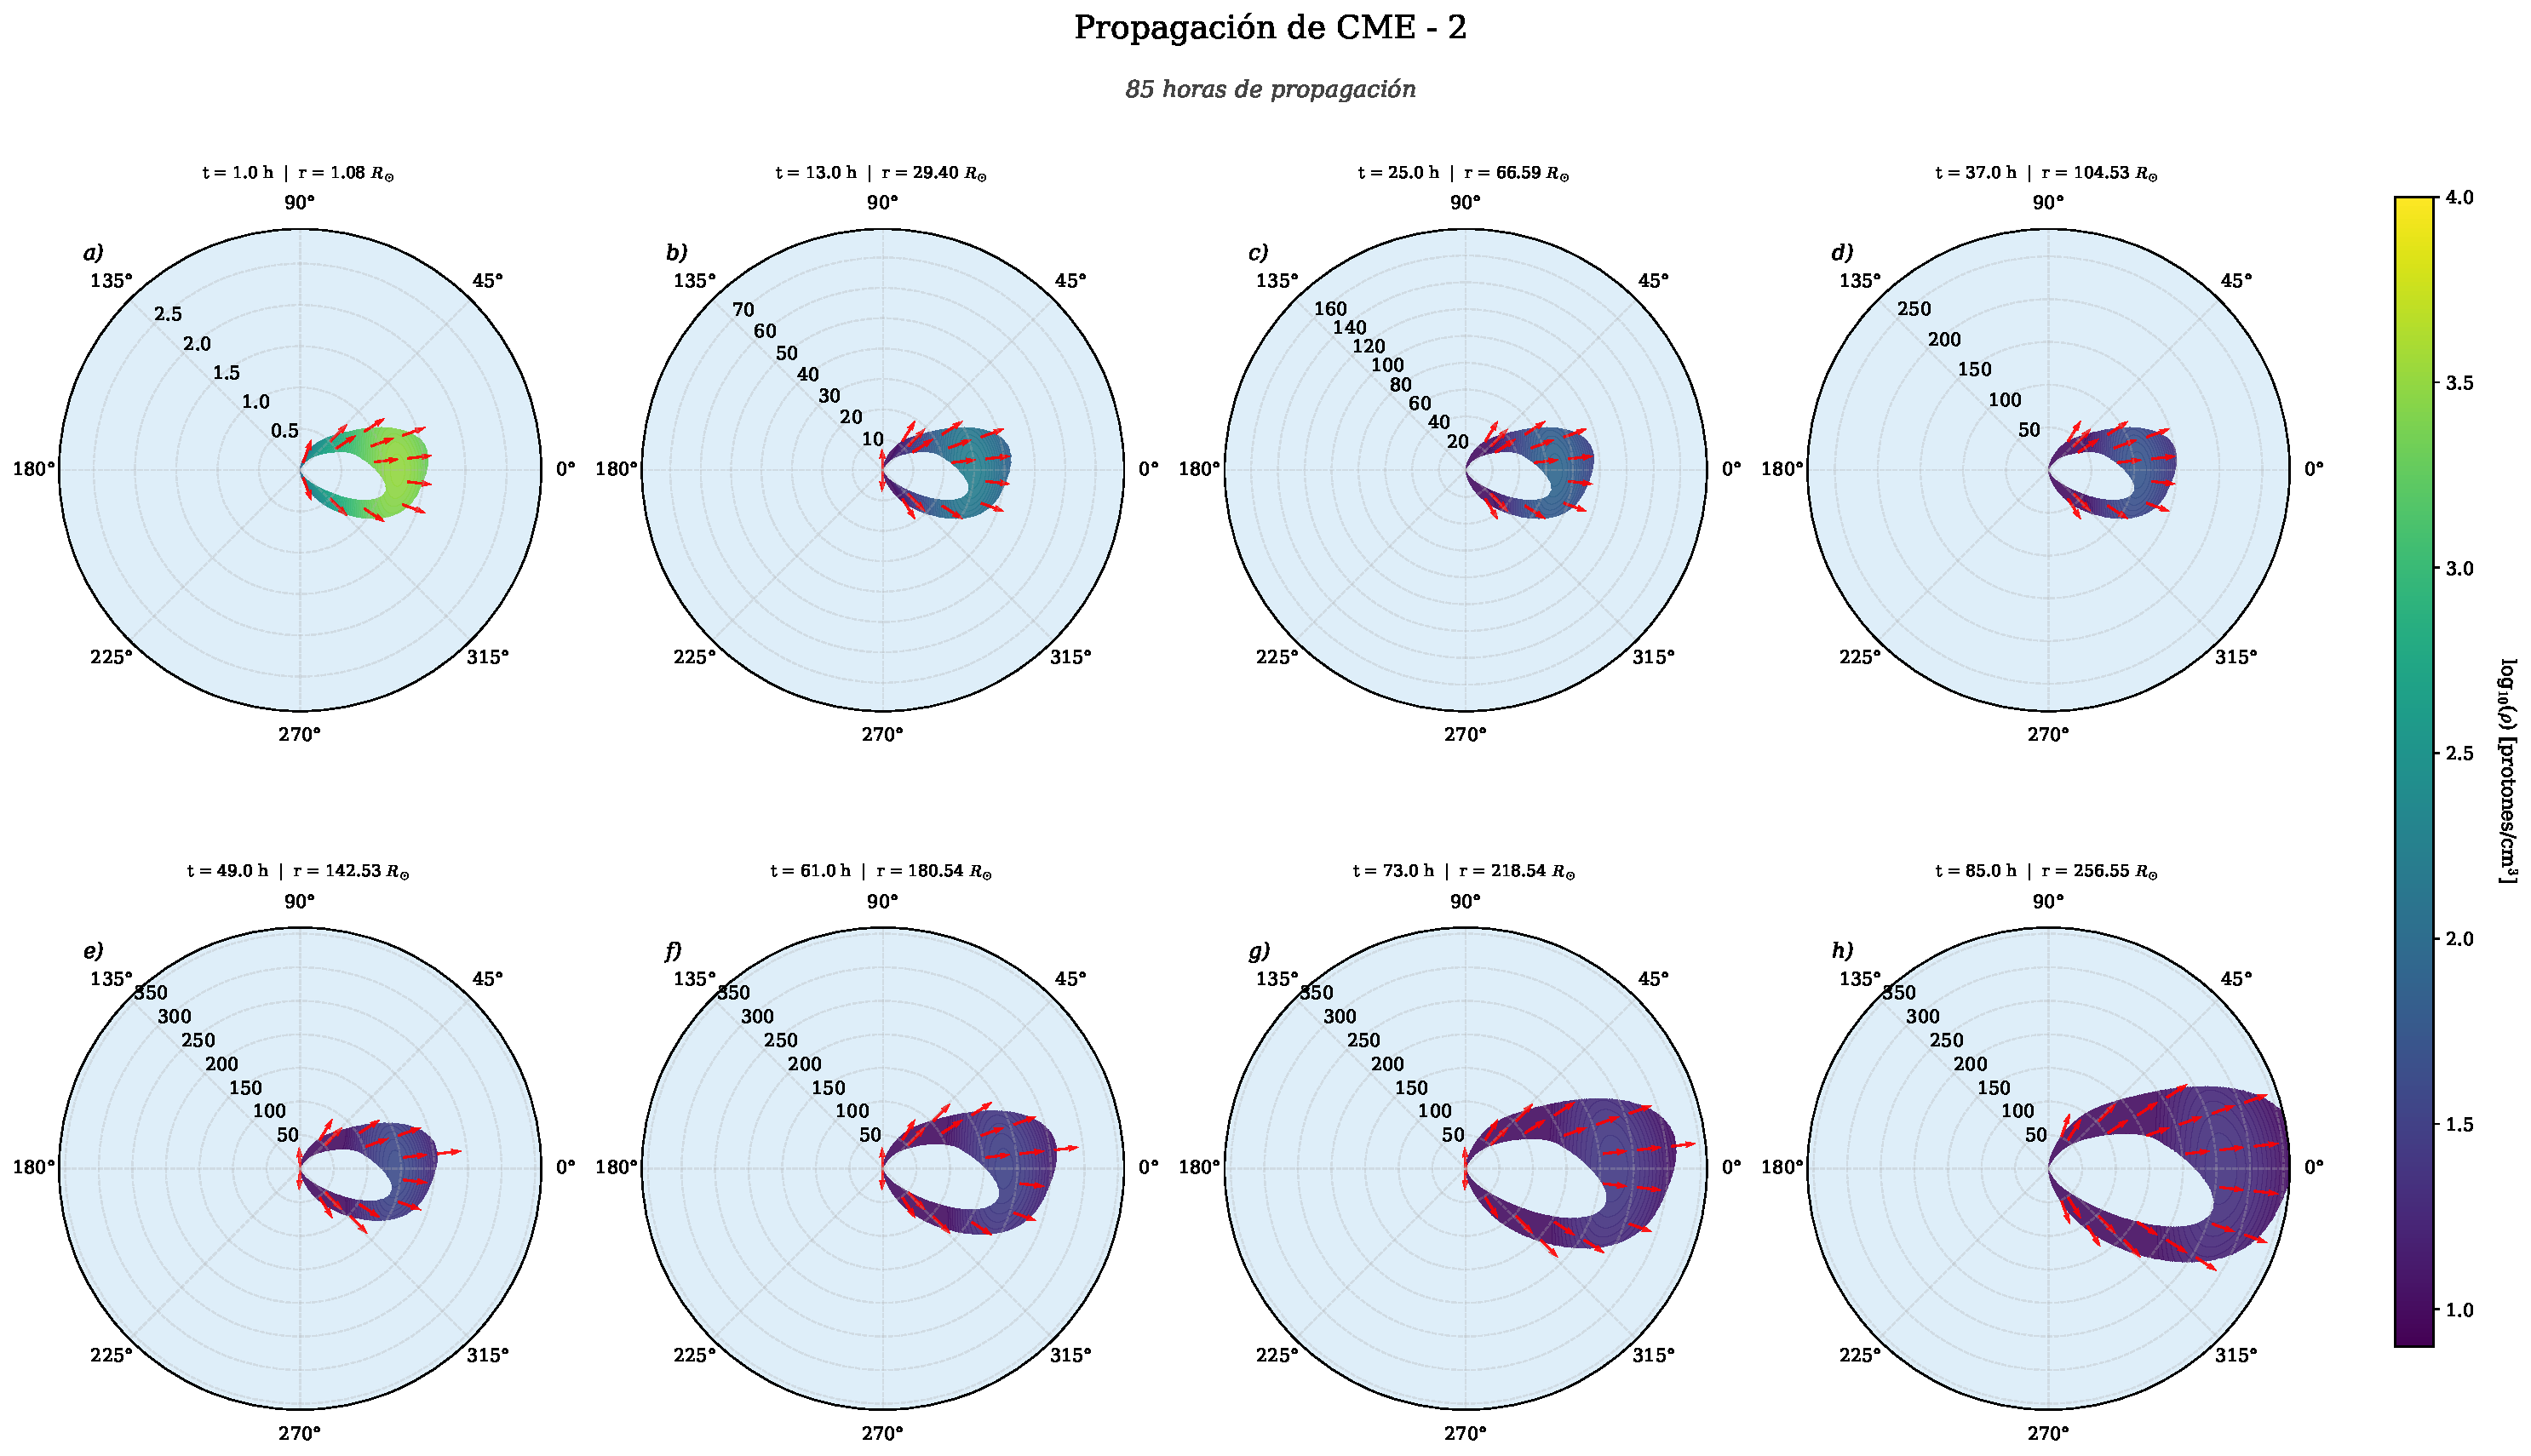
\includegraphics[width=\linewidth]{cme_evolucion_polar_CME2.pdf}
    		\caption[Evolución en 2D de la CME sucesora]{Evolución polar de la CME--2. La escala de colores representa los valores de densidad con mínimos (morado) y máximos (amarillo). La velocidad se indica a través del campo vectorial (rojo). En la parte superior de cada panel se indica el tiempo transcurrido y la posición del centro de la CME.}
    \label{CME2evolución}
	\end{figure}
\end{landscape}

\begin{landscape}
    \begin{figure}[p]
    \centering
    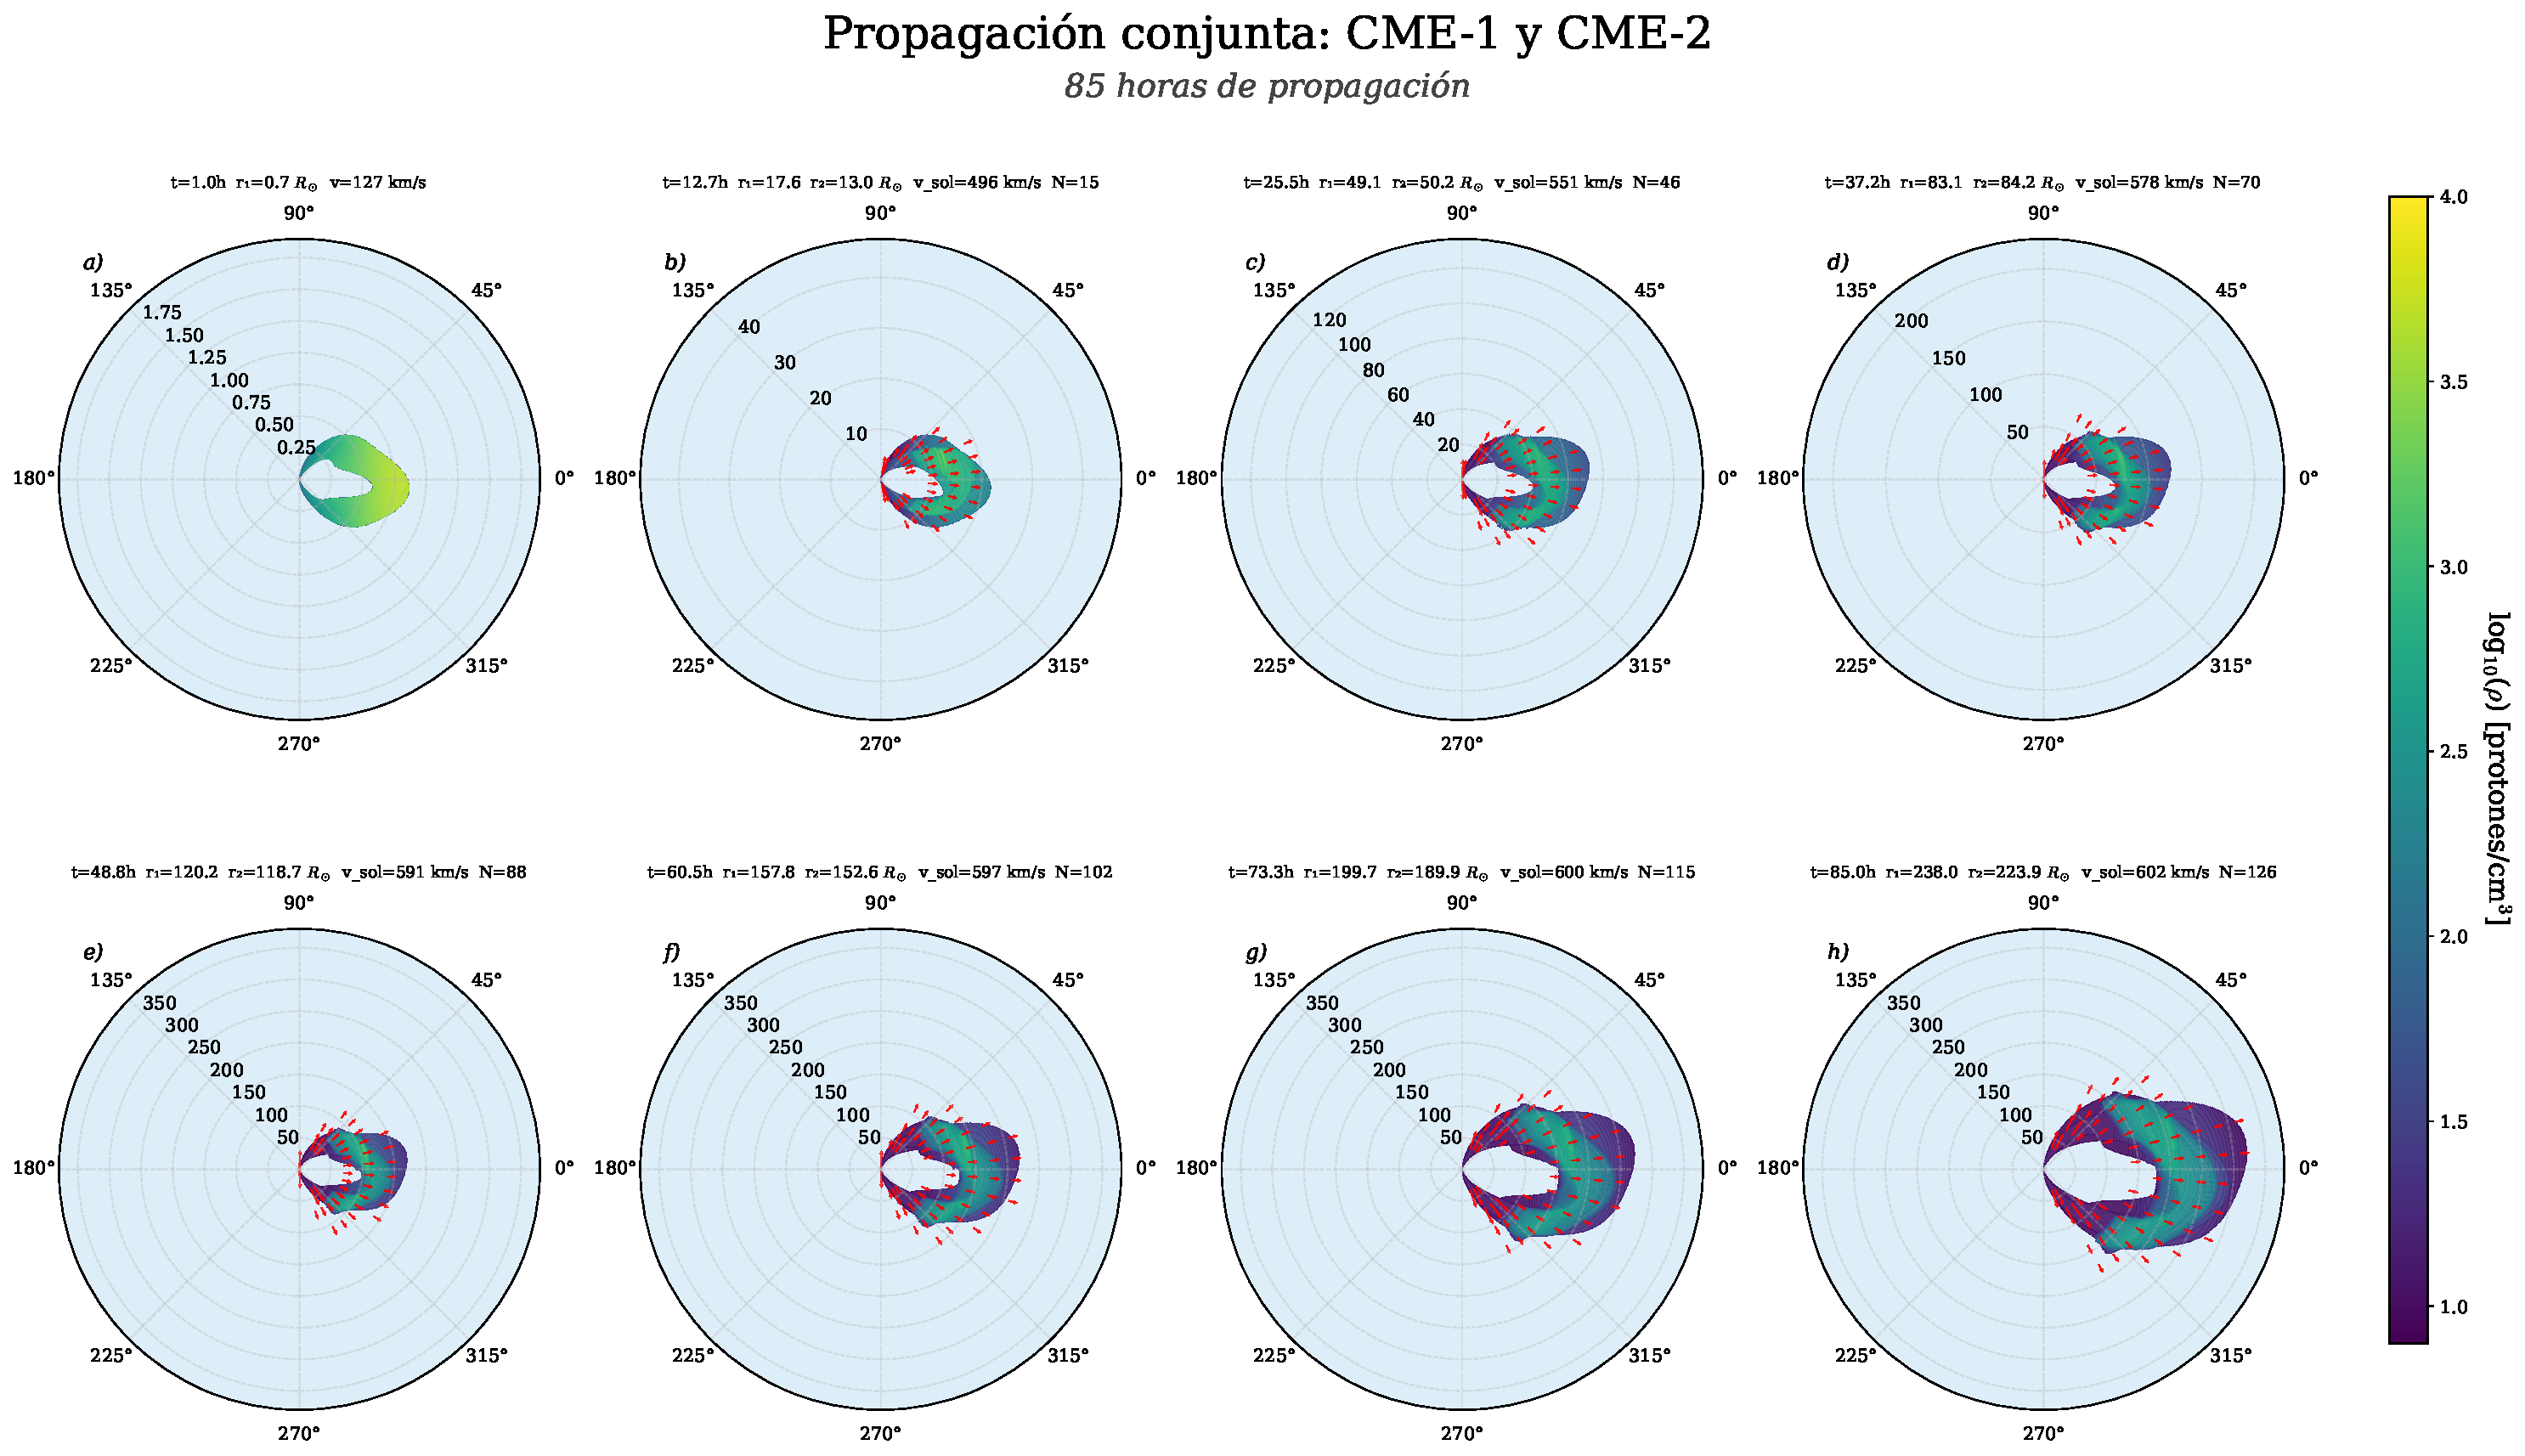
\includegraphics[width=0.95\linewidth]{cme_conjunta_polar_s1_435_s2_1962.pdf}
	\caption[Evolución conjunta de densidad y velocidad de las CMEs en el plano polar para el Caso 1]{Evolución conjunta de densidad y velocidad de las CMEs en el plano polar para el Caso 1. La escala de colores representa los valores de densidad con mínimos (morado) y máximos (amarillo). La magnitud y dirección de la velocidad de las CMEs se muestra a través del campo vectorial (rojo). En la parte superior de cada panel se indica el tiempo de simulación transcurrido junto con la posición del centro de cada CME en ese instante.}
    \label{cinematicapolarconjunta}
    \end{figure}
\end{landscape}

\begin{figure}[h]
    \centering
    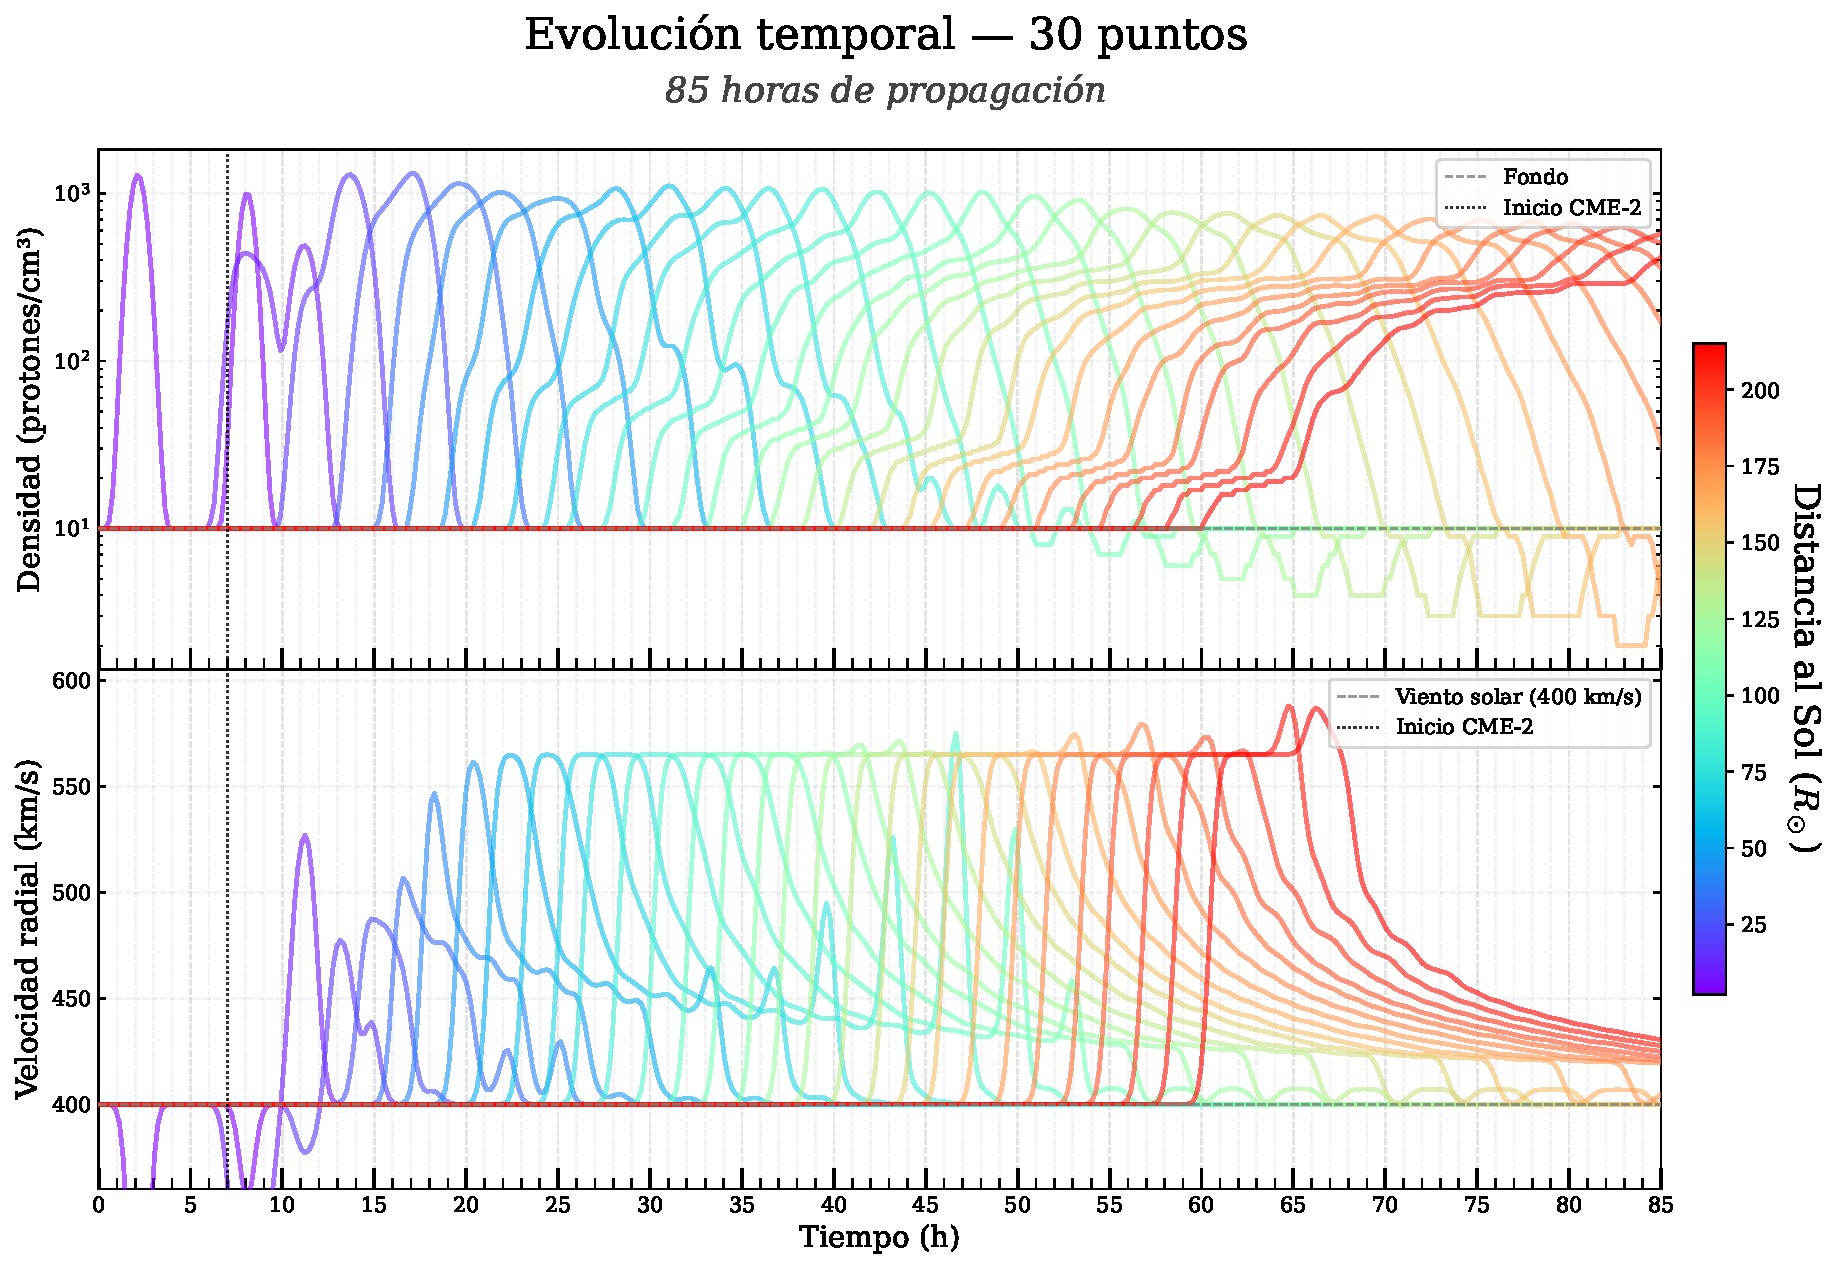
\includegraphics[width=\linewidth]{serie_temporal_multipunto_s1_435_s2_1962.pdf}
    \caption[Series temporales de densidad y velocidad calculados a diferentes distancias para el Caso 1]{Series temporales de densidad (panel superior) y velocidad (panel inferior) para el Caso 1 de interacción, calculadas cerca (morado) y lejos (rojo) del Sol.}
    \label{Serietiempocaso1}
\end{figure}


\section{Resultados de interacción: Caso 2}
Para este caso se toma la misma CME precursora (CME--1) que en el Caso 1, sin embargo se utiliza la CME--3 como sucesora, la cual desarrollando una lenta aceleración en comparación con la CME--2, asimismo se establece un tiempo de retraso de 7 horas entre CMEs. En general, se sigue la misma metodología que en el Caso 1, generando perfiles cinemáticos y mapas de densidad y velocidad, que permiten identificar el comportamiento de su interacción, así como los puntos de interacción en la heliosfera\index{Heliosfera} interna ($\sim1$ AU). De igual manera, se buscan sistemáticamente los parámetros de la CME--3 que favorezcan una interacción con la CME--1, usando el visualizador de perfiles cinemáticos, ver Figura \ref{ejemplosimulación}.

\begin{table}[h]
    \centering
    \footnotesize
    \begin{threeparttable}
        \caption[Valores mínimos de los parámetros $a_d$ y $t_d$ de la CME--3 bajo los cuales hay interacción]{Valores mínimos de los parámetros $a_d$ y $t_d$ de la CME--3 bajo los cuales hay interacción en una región $<1.8$ AU. La CME-1 tarda $\sim 77$ horas $\sim 3,2$ días en llegar a 1,2 AU.}
        \label{tab:parametros_decaimiento2}
        \begin{tabular}{@{}c c c c c c c c@{}}
            \toprule
            \multirow{2}{*}{\#} & $a_d$ & $\tau_d$ & $V_{\text{max}}^{95\%}$ & T int & Altura int & Tiempo $V_{\text{max}}^{95\%}$ & a$_0$ \\
             & (km/s$^2$) & (s) & (km/s) & (h) & (AU) & (h) & (m/s$^2$) \\
            \midrule
            1  & 0,010 & 77521 & 731,92 & 89,70 & 1,180 & 64,66 & 1,66\\
            2  & 0,011 & 70156 & 723,49 & 89,59 & 1,179 & 63,26 & 1,69\\
            3  & 0,012 & 64300 & 710,72 & 89,91 & 1,183 & 59,60 & 1,71\\
            4  & 0,013 & 59700 & 701,71 & 89,55 & 1,178 & 56,59 & 1,73\\
            5  & 0,014 & 55800 & 693,06 & 89,90 & 1,183 & 53,91 & 1,75\\
            6  & 0,015 & 52580 & 687,09 & 89,81 & 1,182 & 51,89 & 1,76\\
            7  & 0,016 & 49820 & 681,29 & 89,82 & 1,182 & 49,87 & 1,78\\
            8  & 0,017 & 47420 & 676,15 & 90,00 & 1,185 & 48,10 & 1,79\\
            9  & 0,018 & 45360 & 672,17 & 89,69 & 1,180 & 46,56 & 1,80\\
            10 & 0,019 & 43510 & 668,38 & 89,83 & 1,182 & 45,22 & 1,81\\
            11 & 0,020 & 41876 & 664,46 & 89,79 & 1,182 & 43,94 & 1,82\\
            12 & 0,021 & 40415 & 662,29 & 89,67 & 1,180 & 42,91 & 1,83\\
            13 & 0,022 & 39085 & 659,43 & 89,80 & 1,182 & 41,87 & 1,83\\
            14 & 0,023 & 37885 & 657,01 & 89,78 & 1,182 & 40,96 & 1,84\\
            15 & 0,024 & 36795 & 654,99 & 89,66 & 1,180 & 40,15 & 1,85\\
            16 & 0,025 & 35785 & 653,02 & 89,84 & 1,182 & 39,43 & 1,85\\
            17 & 0,026 & 34868 & 651,50 & 89,68 & 1,180 & 38,79 & 1,86\\
            18 & 0,027 & 34012 & 649,78 & 89,79 & 1,182 & 38,15 & 1,86\\
            19 & 0,028 & 33222 & 648,07 & 89,79 & 1,182 & 37,51 & 1,87\\
            20 & 0,029 & 32489 & 646,94 & 89,75 & 1,181 & 37,02 & 1,87\\
            21 & 0,1 & 17251 & 620,87 & 89,81 & 1,182 & 26,07 & 1,96 \\
            22 & 0,2 & 13287 & 614,45 & 89,74 & 1,181 & 23,28 & 1,98 \\
            23 & 0,3 & 11647 & 612,07 & 89,60 & 1,179 & 22,17 & 1,97 \\
            24 & 0,4 & 10689 & 611,31 & 89,76 & 1,181 & 21,58 & 1,99 \\
            25 & 0,5 & 10039 & 609,82 & 90,65 & 1,195 & 21,09 & 1,99 \\
            26 & 0,6 & 9559,4 & 609,09 & 90,06 & 1,186 & 20,77 & 1,99 \\
            27 & 0,7 & 9185,37 & 608,62 & 90,01 & 1,185 & 20,53 & 1,99 \\
            28 & 0,8 & 8882,42 & 608,68 & 87,58 & 1,148 & 20,36 & 1,99 \\
            \bottomrule
        \end{tabular}
    \end{threeparttable}
\end{table}

\subsection{Cálculo de perfiles cinemáticos}
Los parámetros de aceleración asignados para la CME--3 consisten en $\tau_r=9560$ s, $a_r=0.002$ km s$^{-2}$, $v_0=140$ km s$^{-1}$ y $x_0=140$ Mm. Luego de buscar los parámetros de aceleración de la CME--3 que favorecen la interacción, se obtiene la Tabla \ref{tab:parametros_decaimiento2}, donde se compila información de los parámetros $a_d$ y $\tau_d$, el valor del 95$\%$ de la velocidad máxima alcanzada ($V_{\text{max}}^{95\%}$) junto con el tiempo en el que se logra, así como la altura y tiempo de la interacción, además de la aceleración inicial (a$_0$). También se genera la Figura \ref{fig:advstd2}, la cual muestra la gráfica de $a_d$ vs $\tau_d$ para este caso, donde la relación no es inversamente proporcional del todo aunque su correlación es muy buena ($R^{2}=0.97$). De igual manera, la Figura \ref{fig:advstdvstodo2} muestra las gráficas de los parámetros de interacción en función de los parámetros cinemáticos $a_d$ (a) y $\tau_d$ (b) de la CME--3, junto a sus curvas de ajuste y coeficientes de correlación, de donde se identifica una baja correlación en algunas gráficas.

\begin{figure}[h]
    \centering
    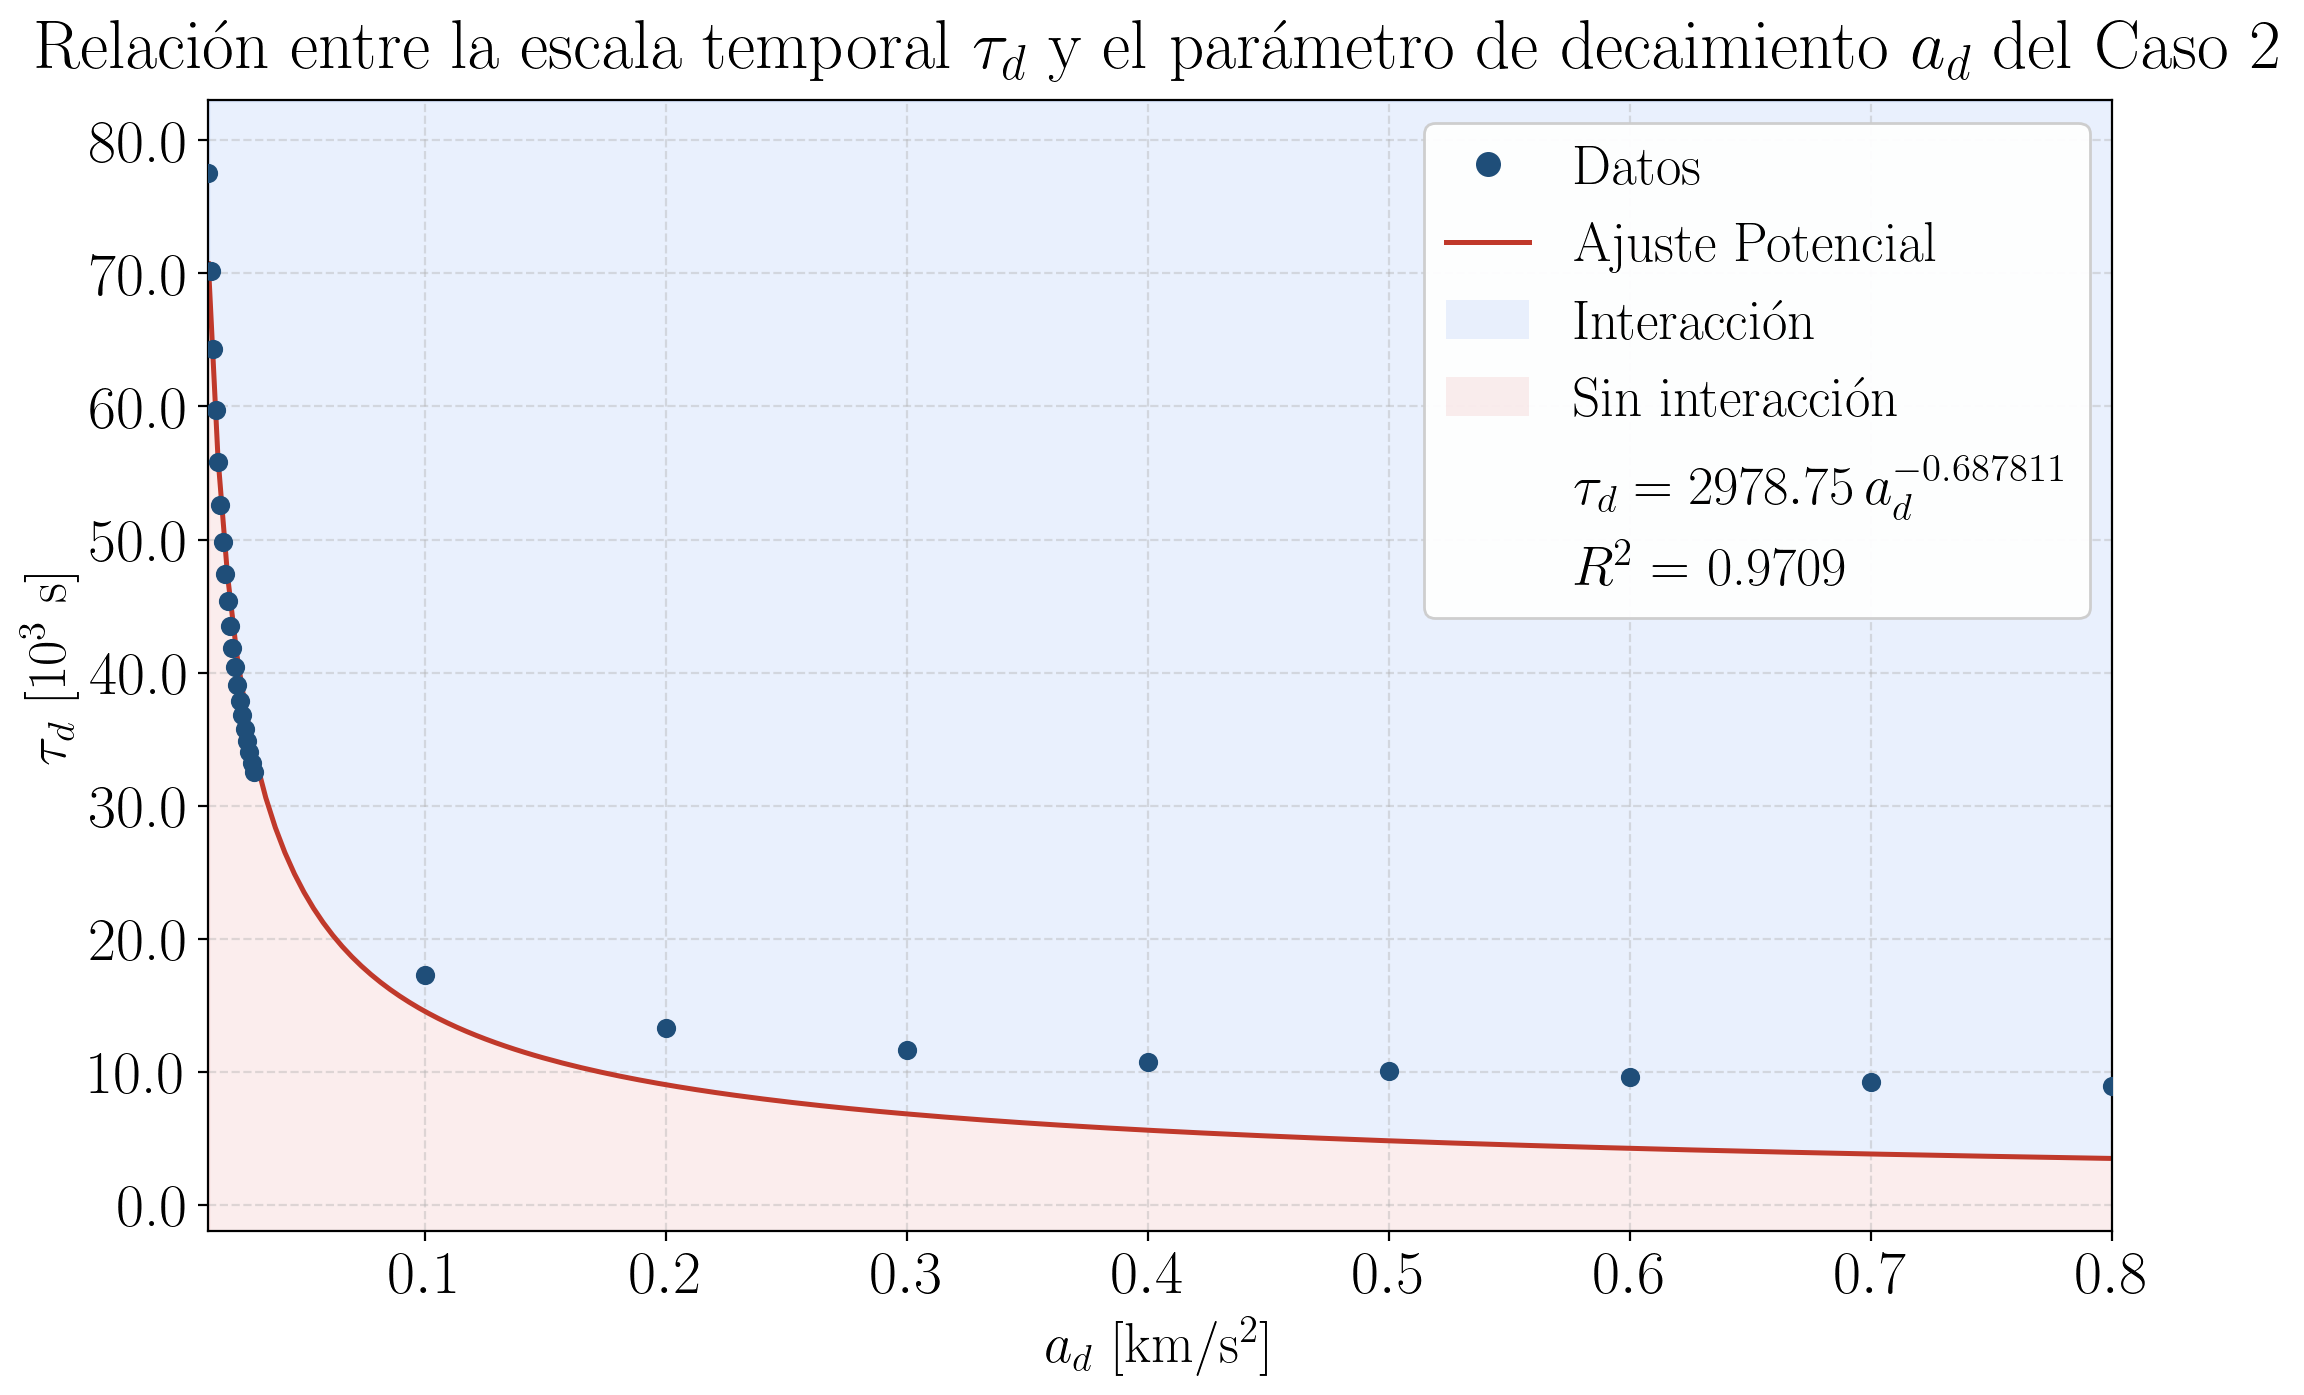
\includegraphics[width=\linewidth]{resultados/fig_ad_vs_td2.png}
    \caption[Gráfica de $a_d$ vs $\tau_d$ para el Caso 2]{Gráfica de $a_d$ vs $\tau_d$ para el Caso 2, junto a la curva de ajuste (línea roja), ecuación característica y coeficiente de correlación, delimitando una región de interacción (azul) de una región en donde no la hay (roja). Los puntos en azul son los datos de la CME sucesora donde ocurre la interacción.}
    \label{fig:advstd2}
\end{figure}


\begin{figure}[htbp]
    \centering
    \begin{subfigure}{\textwidth}
        \centering
        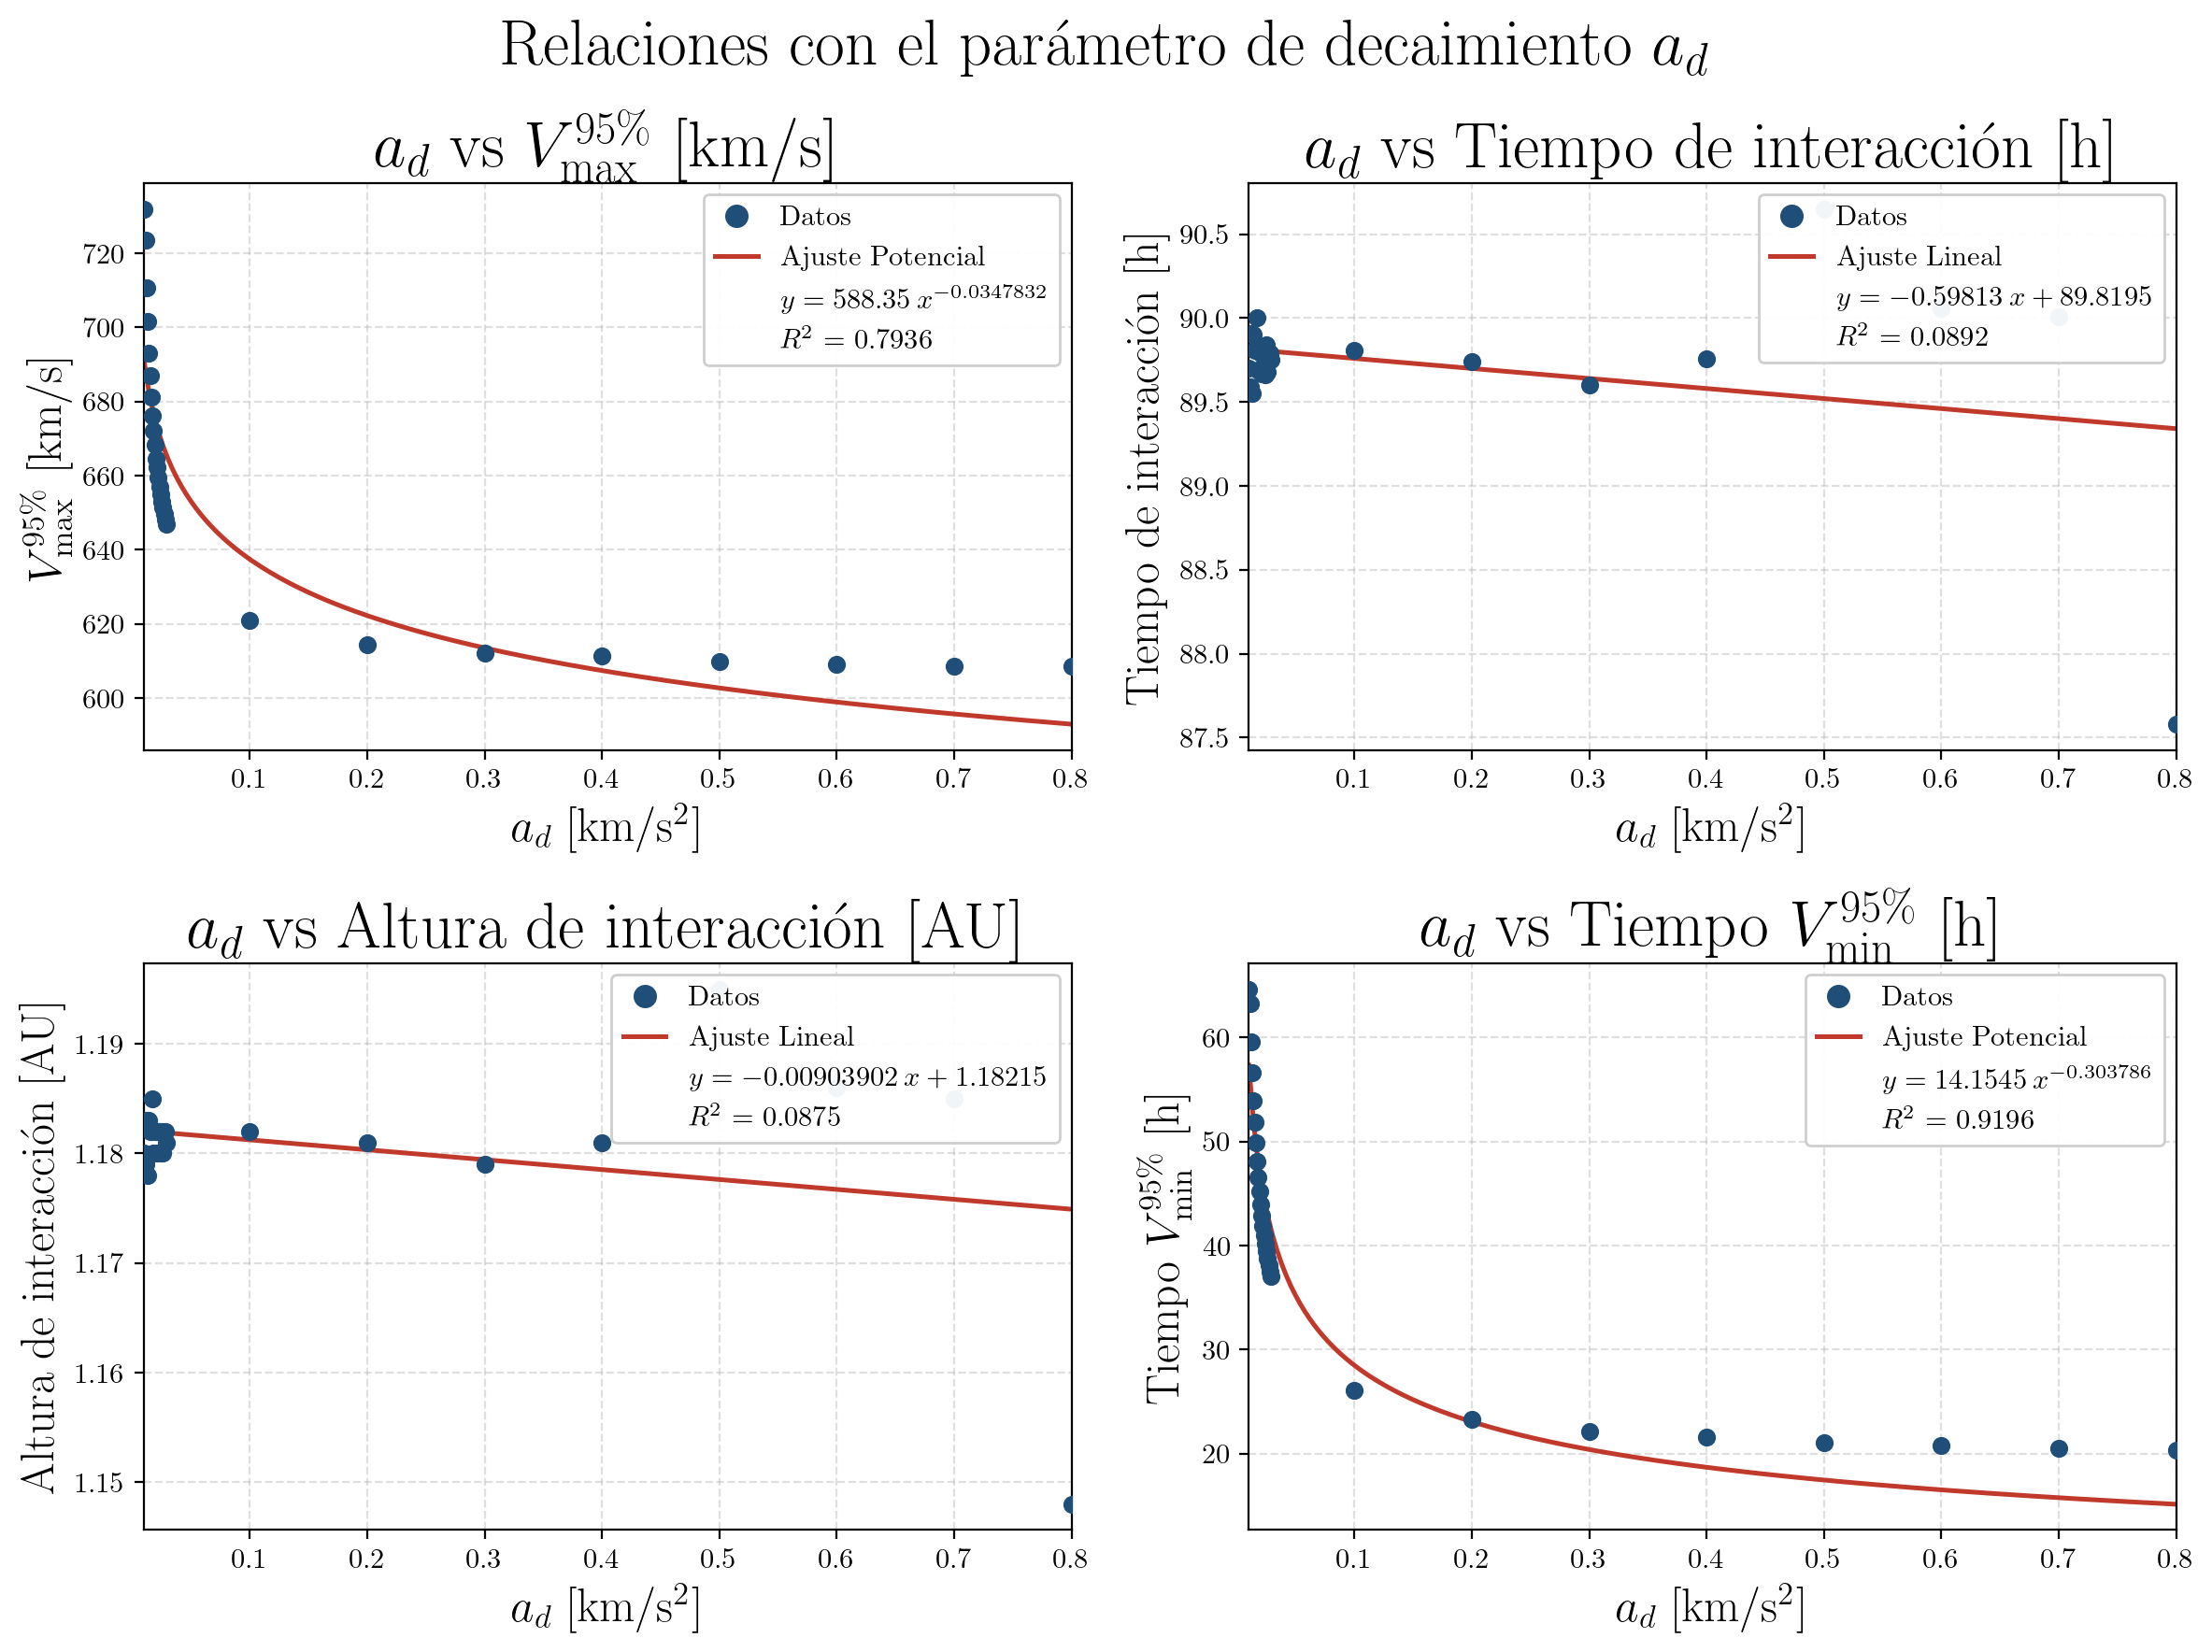
\includegraphics[width=0.9\linewidth]{resultados/fig_ad_relaciones2.png}
        \caption*{(a)}
    \end{subfigure}
    \hfill
    \begin{subfigure}{\textwidth}
        \centering
        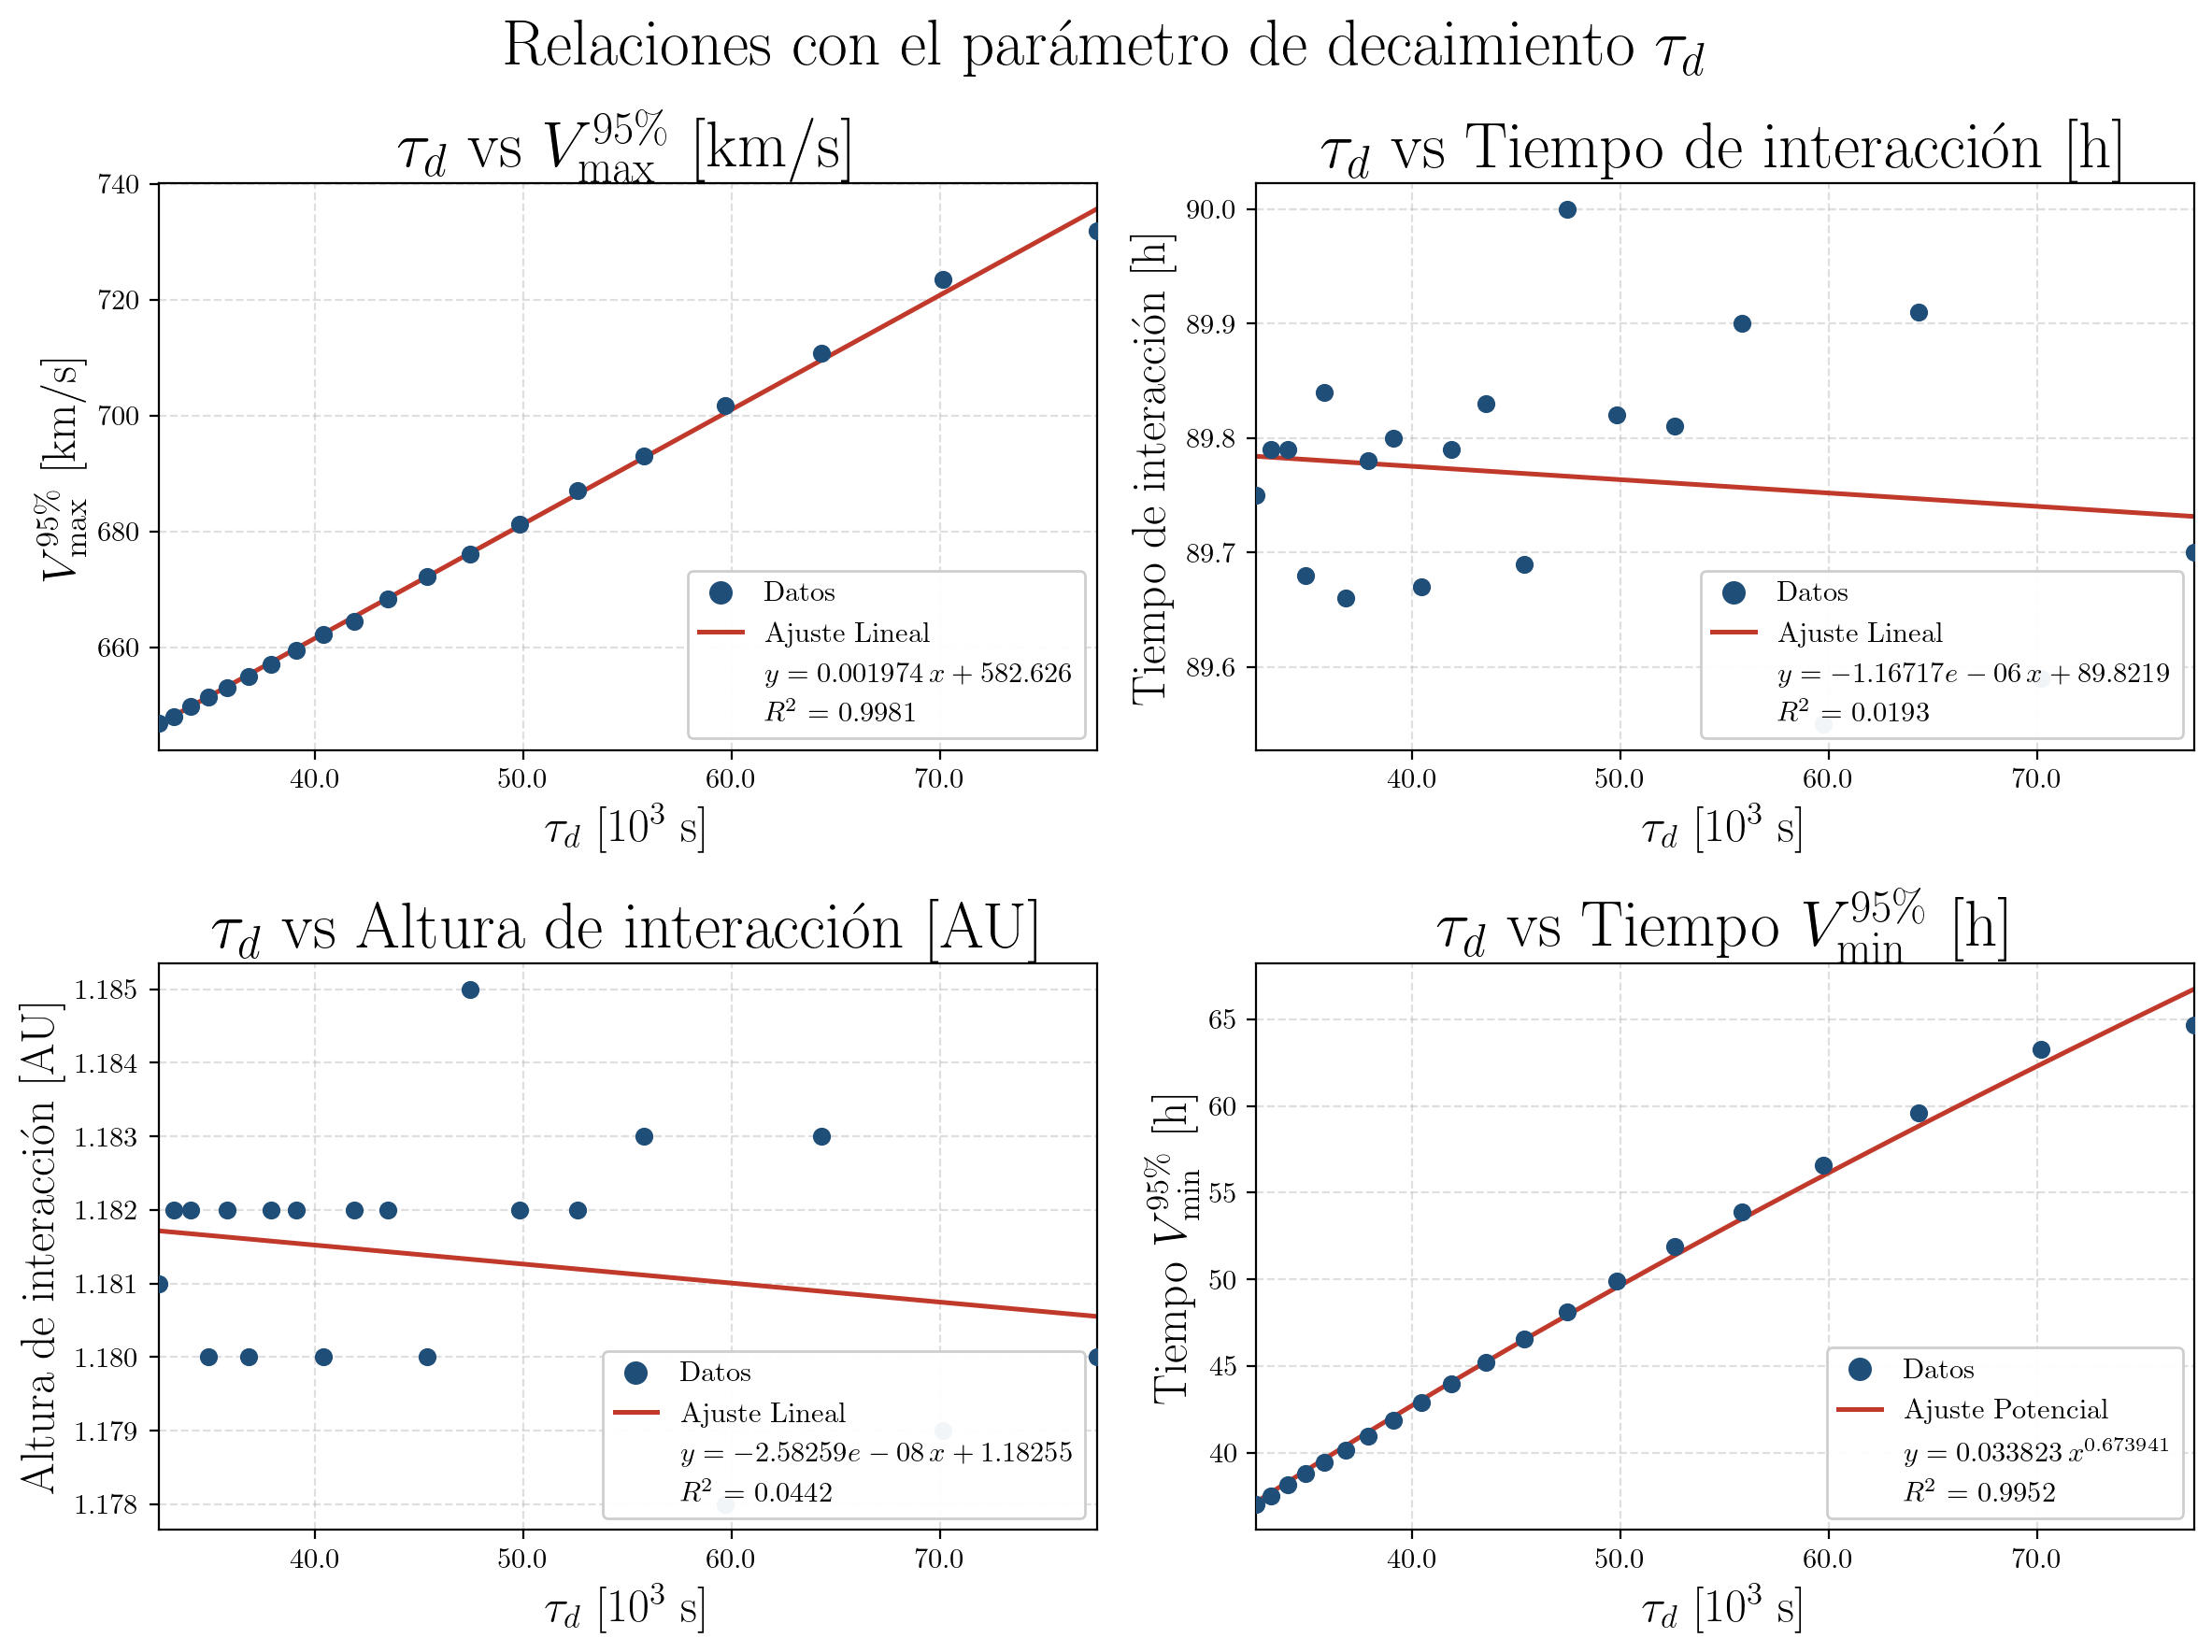
\includegraphics[width=0.9\linewidth]{resultados/fig_td_relaciones2.png}
        \caption*{(b)}
    \end{subfigure}
    \caption[Gráficas de $a_d$ y $\tau_d$ vs parámetros de interacción para el Caso 2]{Gráficas de $a_d$ (a) y $\tau_d$ (b) vs parámetros de interacción para el Caso 2, junto a las curvas de ajuste (línea roja) correspondientes, ecuaciones características y coeficientes de correlación. Los puntos en azul son los datos de la CME--3 bajo los cuales ocurre la interacción.}
    \label{fig:advstdvstodo2}
\end{figure}

De la misma manera que se generan los perfiles cinemáticos para las CMEs del Caso 1, en la Figura \ref{cinematicaconjunta2} se muestran los perfiles de la CME--1 y de la CME--3 del evento $\#28$ de la Tabla \ref{tab:parametros_decaimiento2}. Al comparar con la Figura \ref{cinematicaconjunta}, es evidente la diferencia en la duración de la fase de aceleración de la CME--3 con respecto a la CME--2.

\begin{figure}[h]
    \centering
    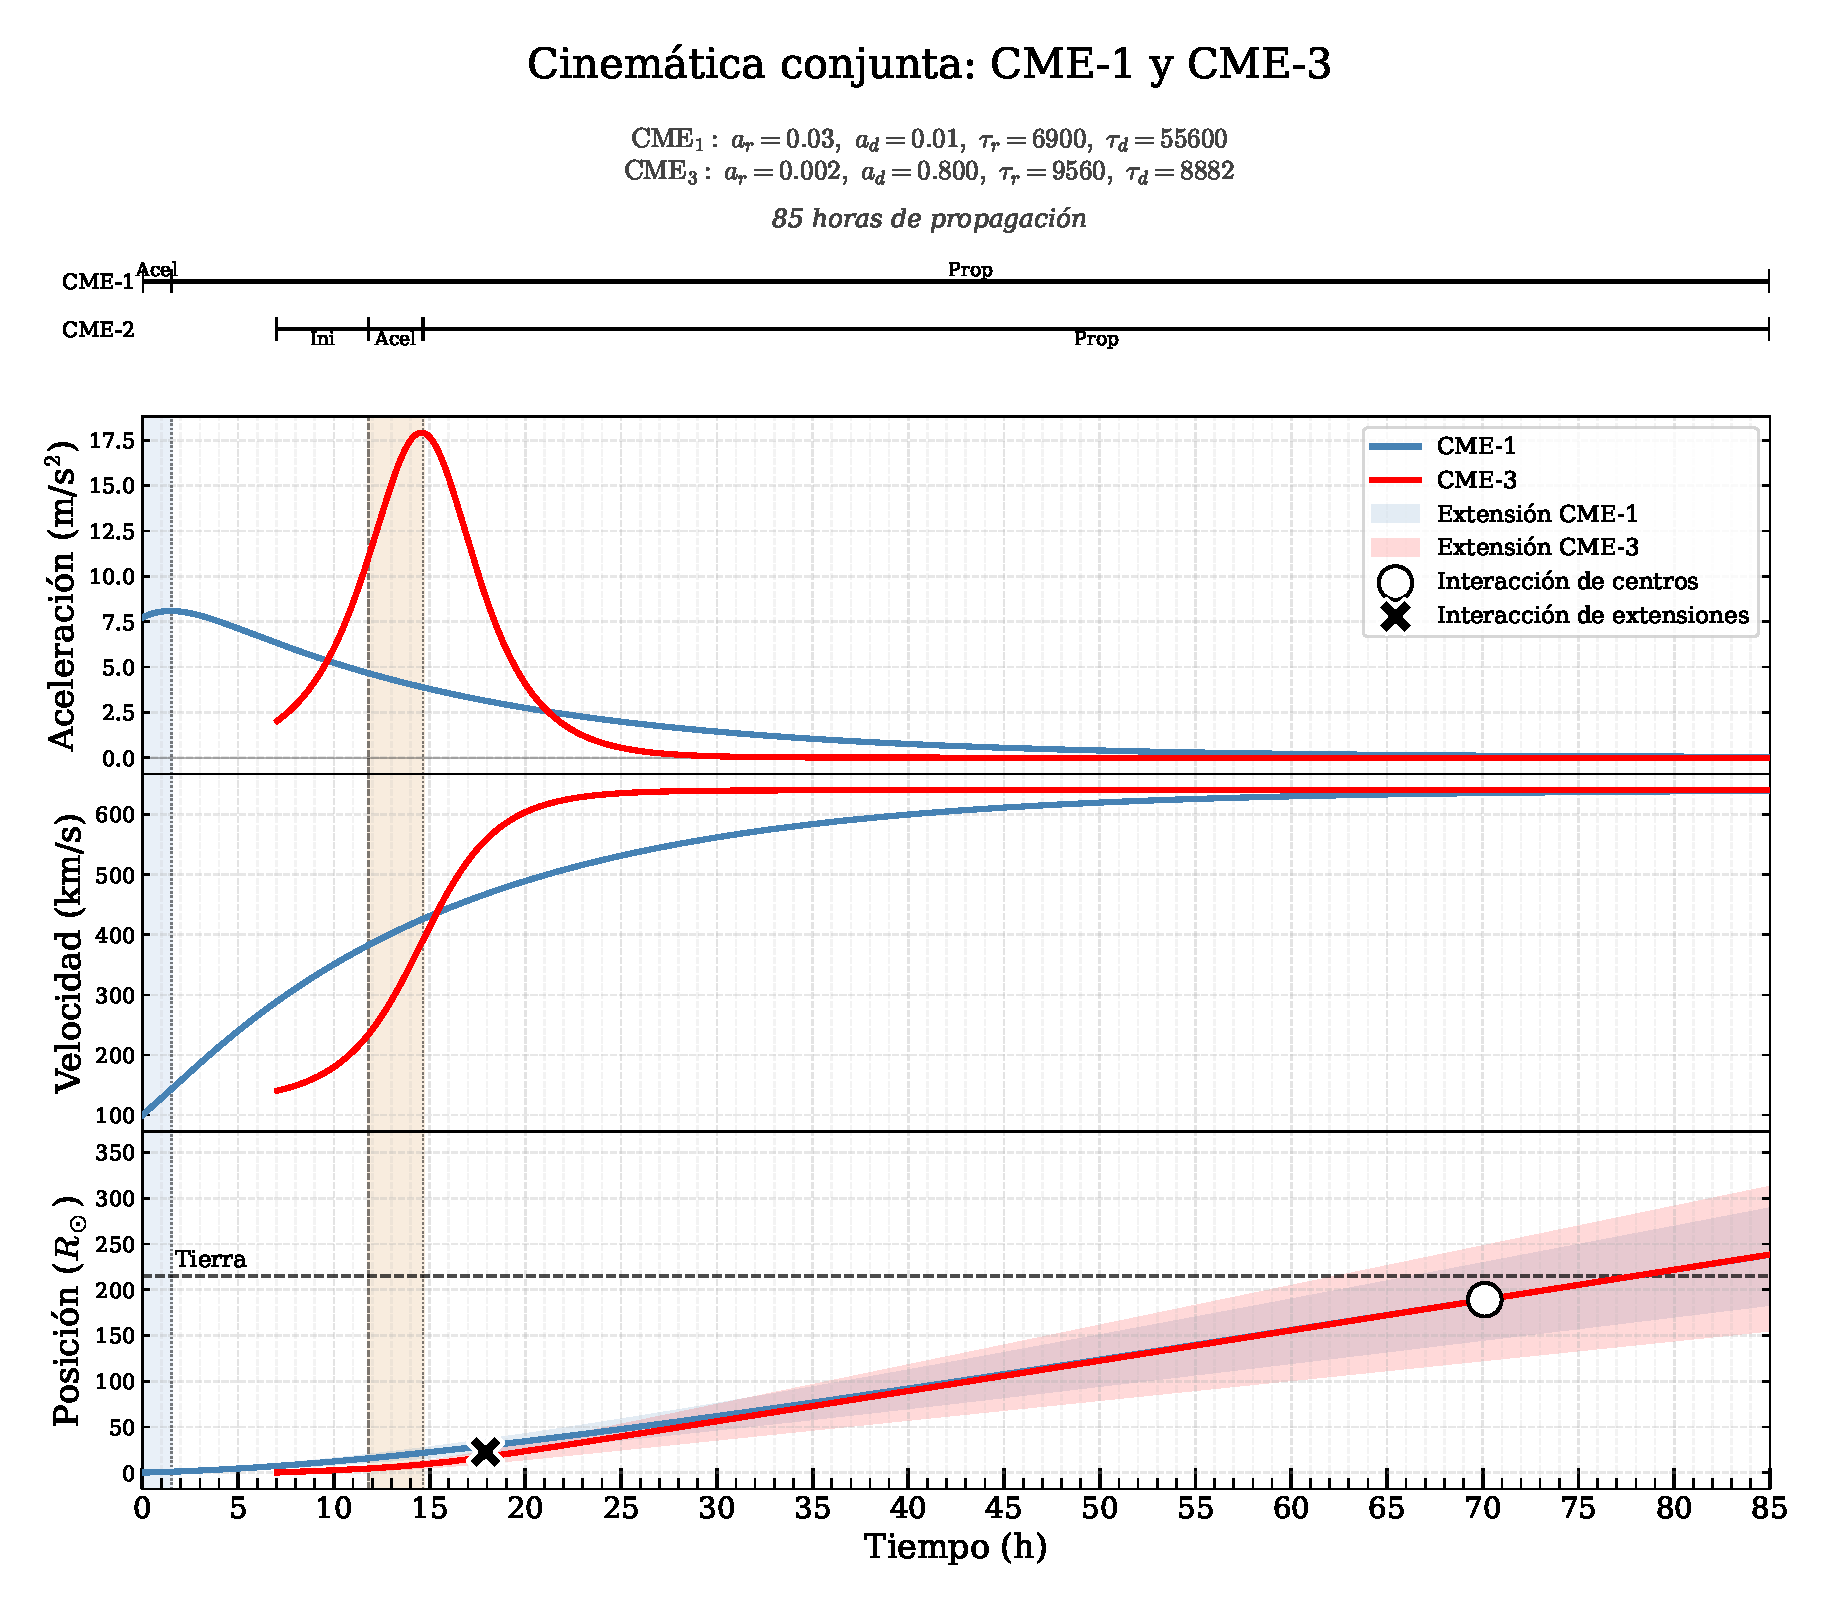
\includegraphics[width=\linewidth]{cinematica_conjunta_s1_435_s2_256_2.pdf}
    \caption[Perfiles cinemáticos de las dos CMEs sin interacción]{Perfiles cinemáticos de la CME--1 (azul) y CME--3 (rojo) sin considerar interacción. Además se señalan las etapas de aceleración: iniciación (Ini), aceleración (Acel) y propagación (Prop) respectivamente para la CME--1 y 3. Además, las etapas de iniciación y aceleración están separadas por una línea discontinua, mientras que las etapas de aceleración y propagación lo están con una línea punteada. La expansión de las CMEs se muestra como la región sombreada que envuelve la curva de posición de su centro. La posición de la Tierra se muestra con una línea discontinua horizontal.}
    \label{cinematicaconjunta2}
\end{figure}

\subsection{Cálculo de densidad y velocidad de la interacción}
Se utiliza la CME--1 mostrada en la Figura \ref{CME1evolución} y la CME--3 mostrada en la Figura \ref{CME2evolución2}. De igual manera, la Figura \ref{cinematicapolarconjunta2} muestra la evolución conjunta de las CMEs en el plano polar, la cual describe un incremento en la densidad de la misma manera que para el Caso 1, ver Figura \ref{cinematicapolarconjunta}. Asimismo, se calculan las series temporales de densidad y velocidad, como lo muestra la Figura \ref{Serietiempocaso2}, usando la misma densidad y velocidad de fondo que para el caso previo (10 protones cm$^{-3}$, 400 km s$^{-1}$).

\section{Análisis de resultados}
\label{análisisderesultados}
La curva de ajuste $\tau_d$ vs $a_d$ presenta una pendiente menos pronunciada cerca del origen en el Caso 2 (Figura \ref{fig:advstd2}) en comparación con el Caso 1 (Figura \ref{fig:advstd}), lo que se traduce en una región de parámetros ($a_d,\tau_d$) en la cual la interacción es favorable más amplia para el Caso 1, en relación con el Caso 2. Por lo tanto, se esperaría que la interacción sea más probable cuando la CME sucesora presenta una aceleración abrupta que cuando esta es suave, ya que una aceleración abrupta le permite alcanzar velocidades máximas en menos tiempo en comparación con una suave. El Caso 1 (Caso 2) presenta distancias de interacción menores a $\sim0{,}25$ AU ($\sim1{,}15$ AU) siempre que la CME sucesora alcance una velocidad mínima de $\sim520$ km s$^{-1}$ ($\sim666$ km s$^{-1}$) en menos de $\sim11$ horas ($\sim51$ horas), mientras que a distancias mayores a $\sim0{,}25$ AU ($\sim1{,}15$ AU), la CME precursora ya no puede ser alcanzada por la sucesora. 

\begin{landscape}
    \begin{figure}[p]
        \centering
        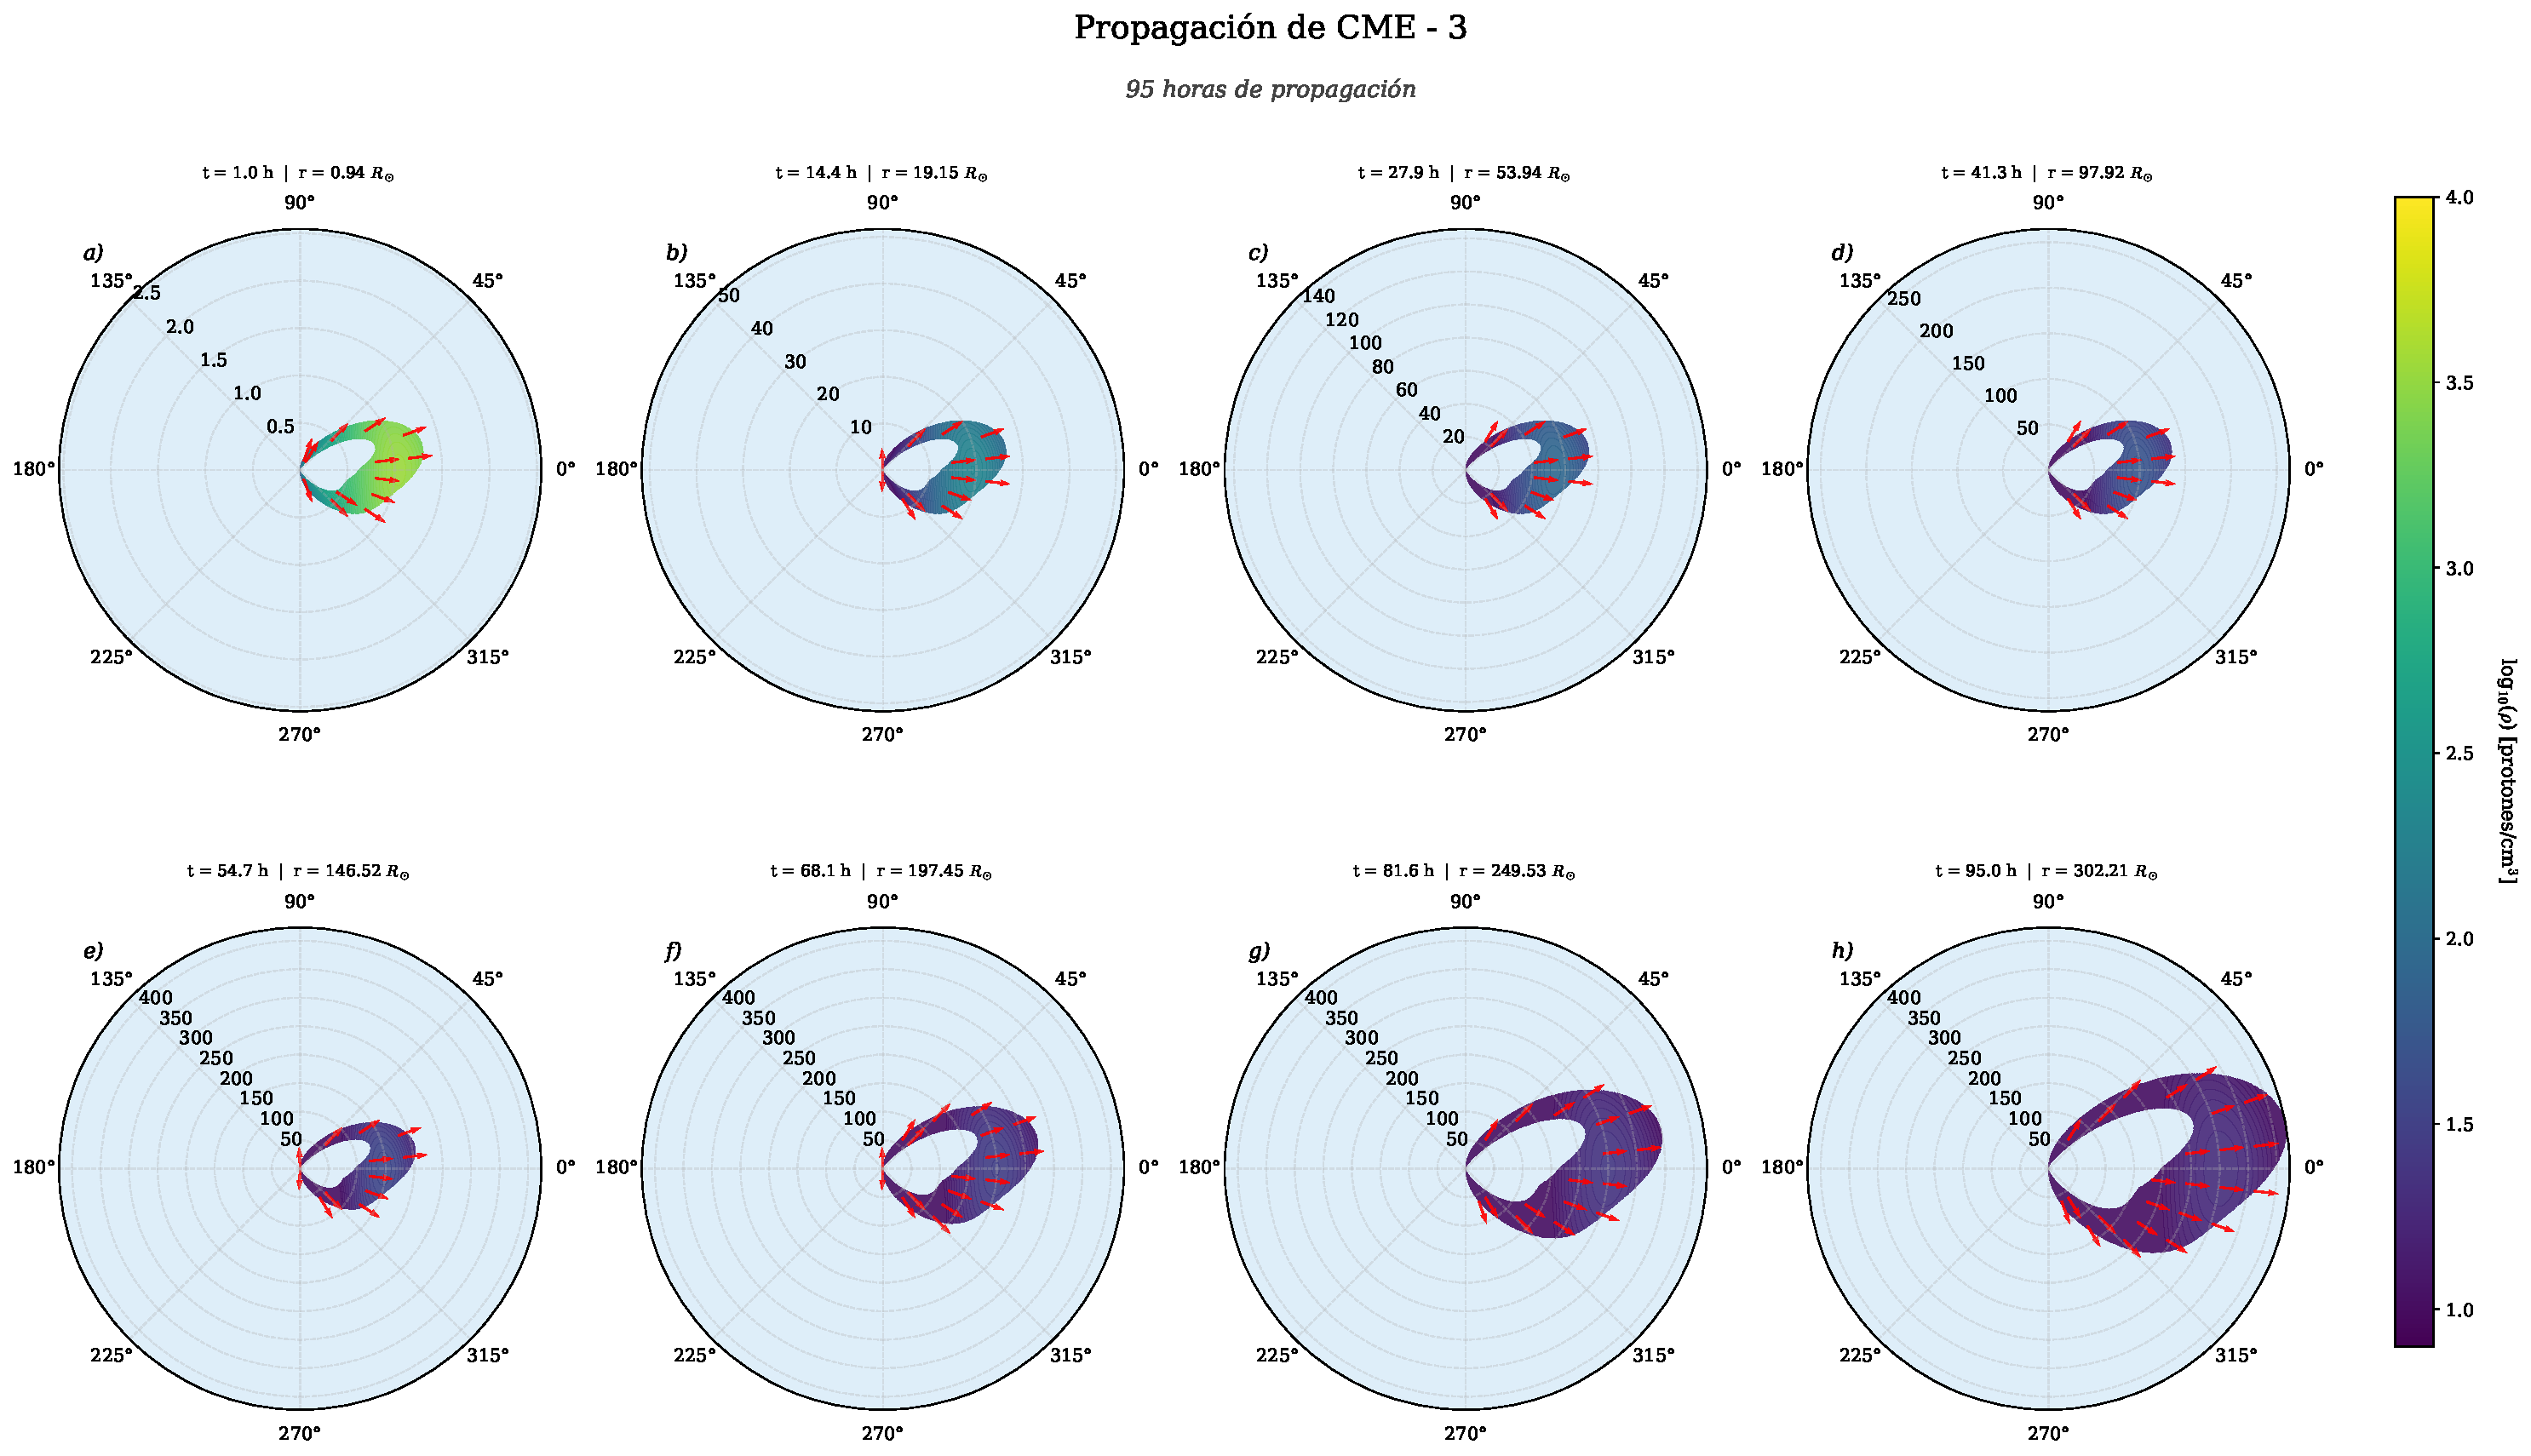
\includegraphics[width=\linewidth]{cme_evolucion_polar_CME3.pdf}
    		\caption[Evolución en 2D de la CME sucesora]{Evolución polar de la CME--3. La escala de colores representa los valores de densidad con mínimos (morado) y máximos (amarillo). La velocidad se indica a través del campo vectorial (rojo). En la parte superior de cada panel se indica el tiempo transcurrido y la posición del centro de la CME.}
    \label{CME2evolución2}
	\end{figure}
\end{landscape}
\begin{landscape}
    \begin{figure}[p]
    \centering
    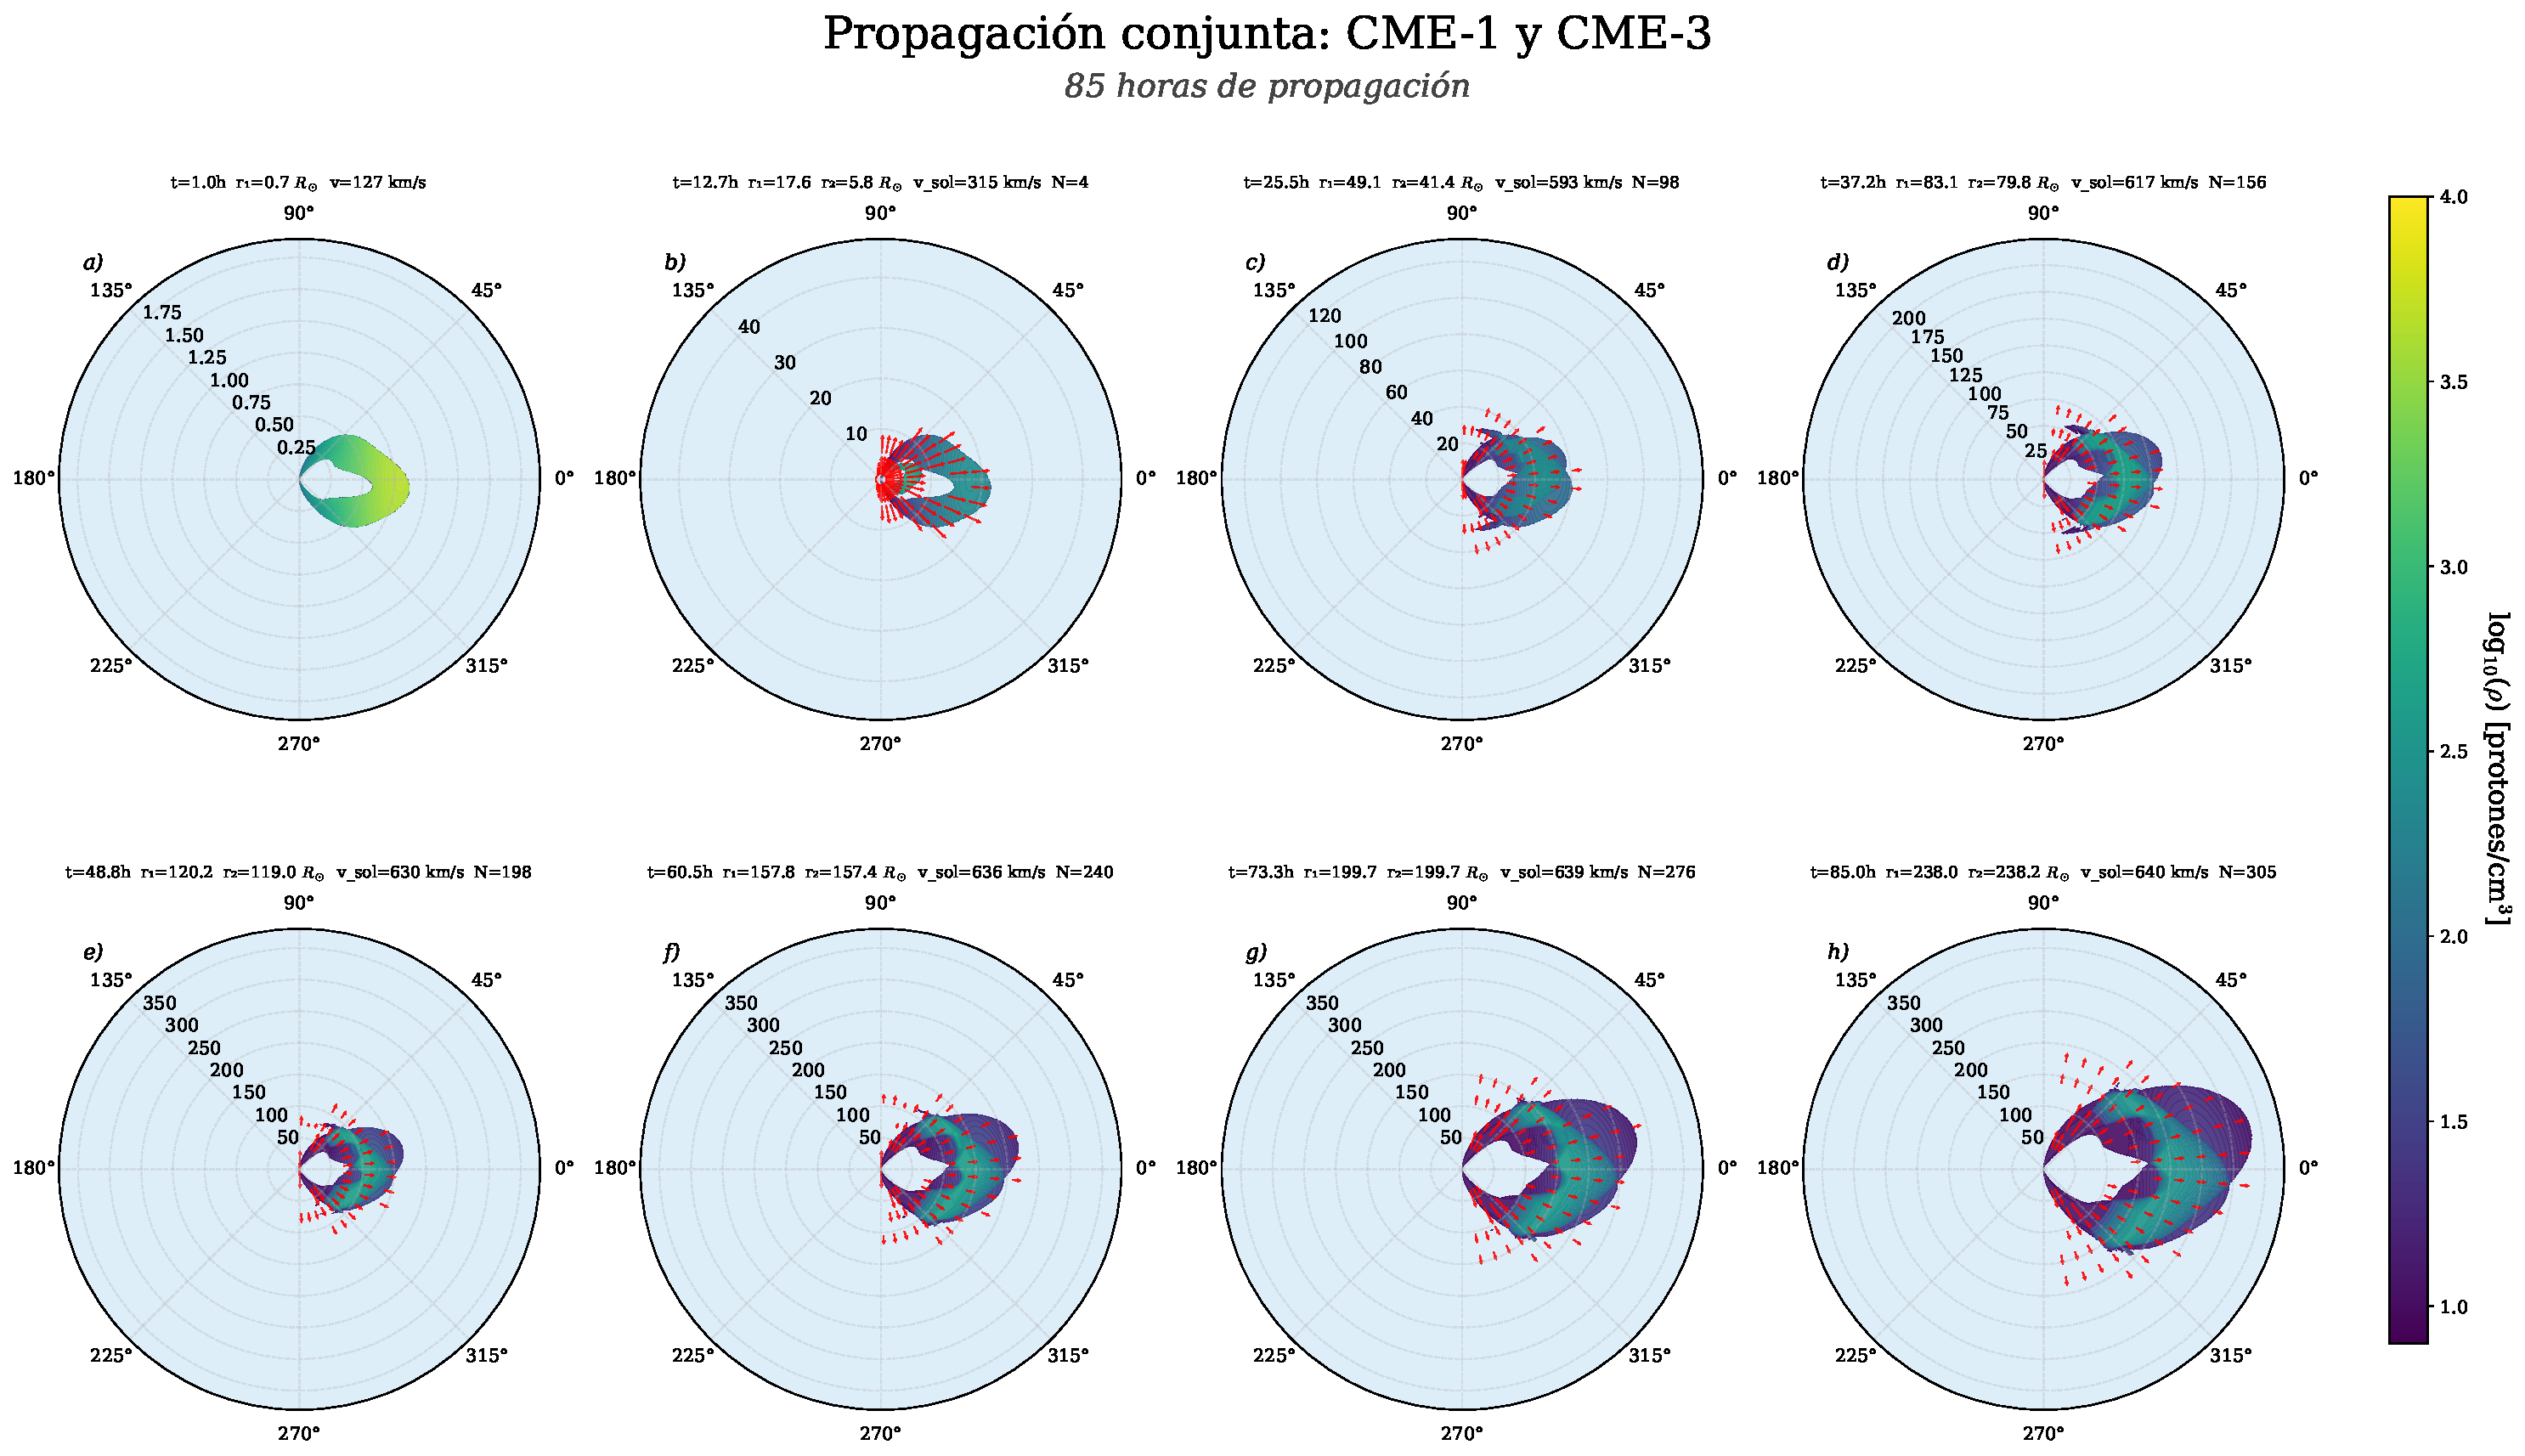
\includegraphics[width=0.95\linewidth]{cme_conjunta_polar_s1_435_s2_256_2.pdf}
	\caption[Evolución conjunta de densidad y velocidad de las CMEs en el plano polar para el Caso 2]{Evolución conjunta de densidad y velocidad de las CMEs en el plano polar para el Caso 2. La escala de colores representa los valores de densidad con mínimos (morado) y máximos (amarillo). La magnitud y dirección de la velocidad de las CMEs se muestra a través del campo vectorial (rojo). En la parte superior de cada panel se indica el tiempo de simulación transcurrido junto con la posición del centro de cada CME en ese instante.}
    \label{cinematicapolarconjunta2}
    \end{figure}
\end{landscape}

\begin{figure}[h]
    \centering
    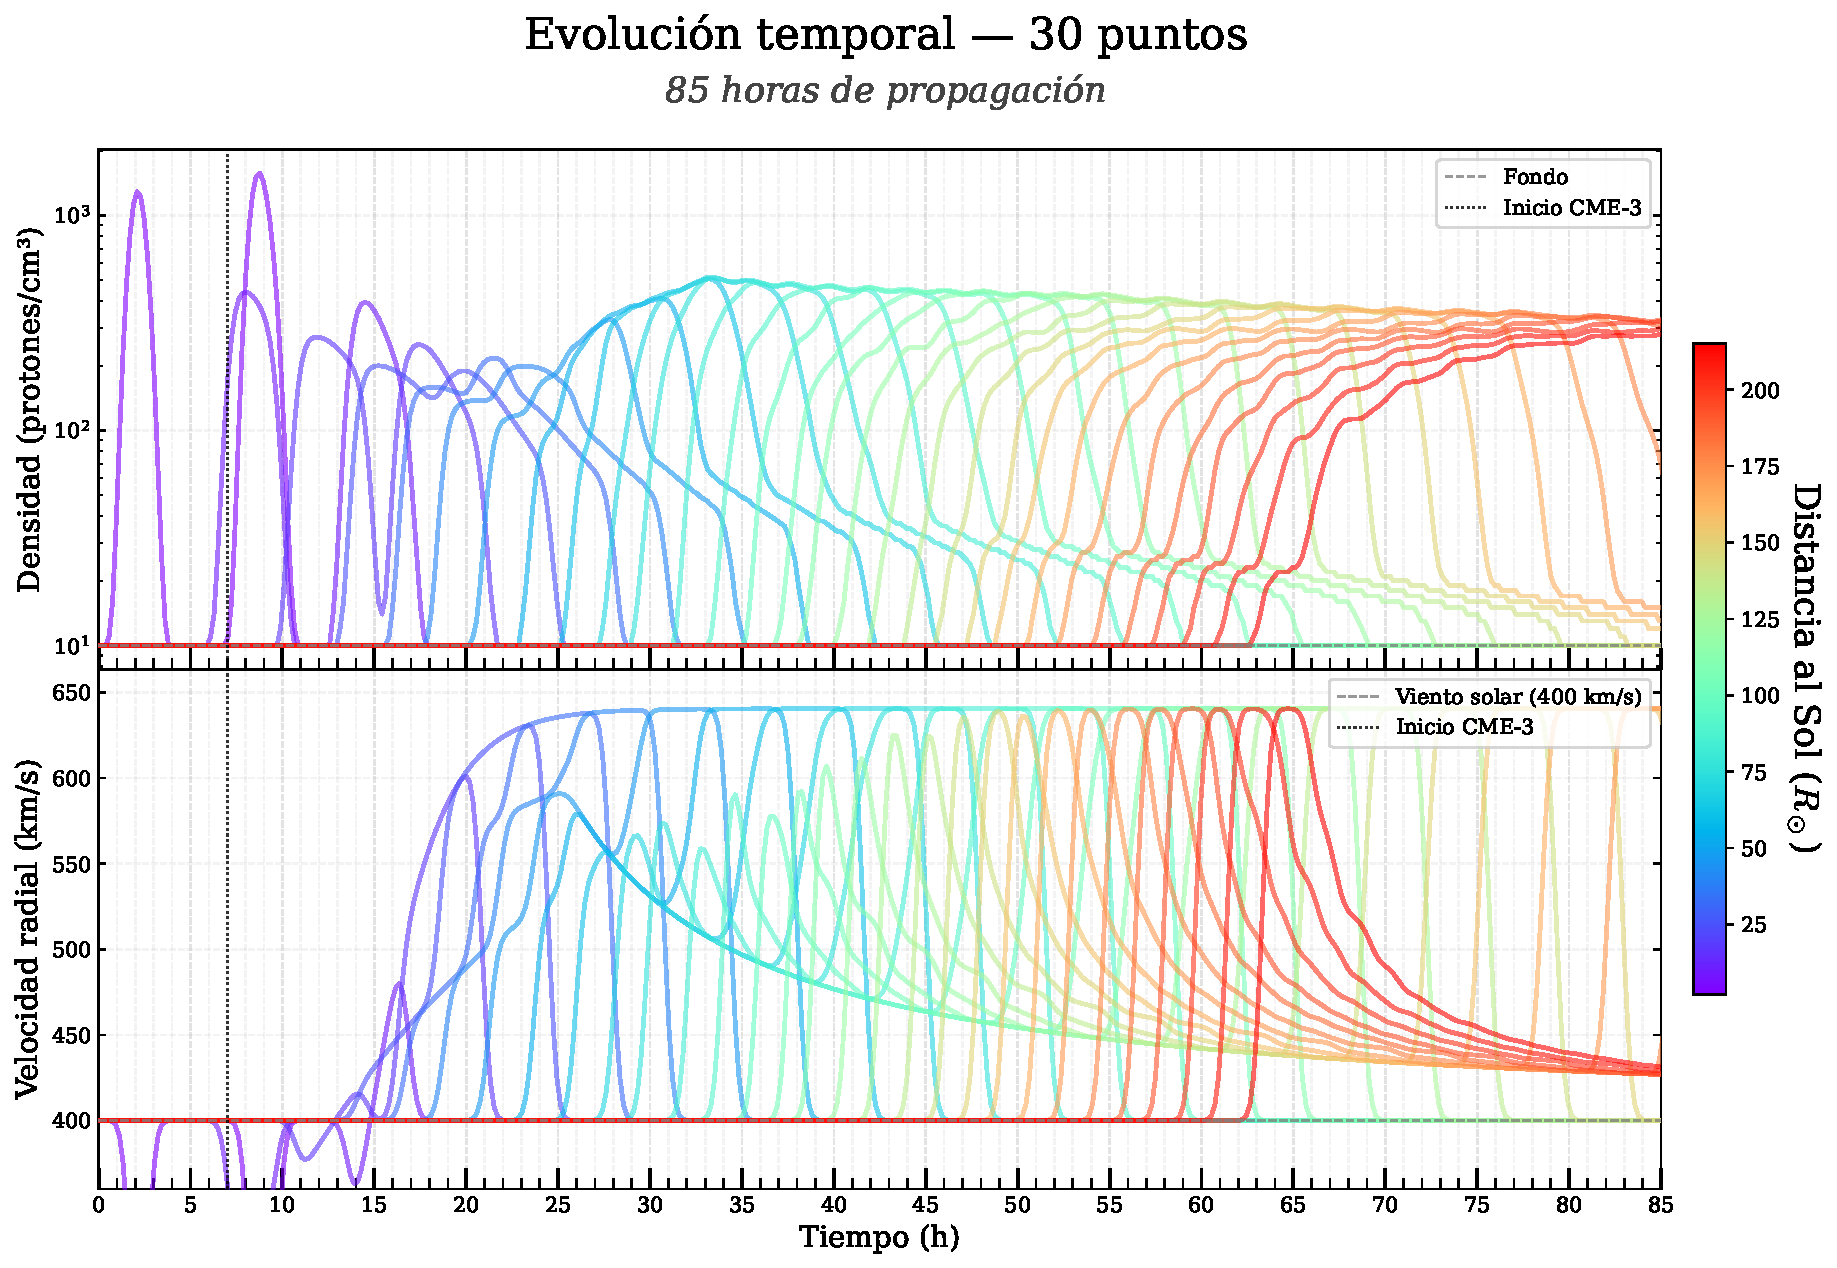
\includegraphics[width=\linewidth]{serie_temporal_multipunto_s1_435_s2_256_2.pdf}
    \caption[Series temporales de densidad y velocidad calculados a diferentes distancias para el Caso 2]{Series temporales de densidad (panel superior) y velocidad (panel inferior), calculadas cerca (morado) y lejos (rojo) del Sol, para el Caso 2 de interacción.}
    \label{Serietiempocaso2}
\end{figure}

Para que la interacción sea altamente probable, bajo los parámetros cinemáticos de las CMEs previamente fijados, se deben cumplir los siguientes umbrales. Un primer criterio surge de la razón entre las velocidades de la CME sucesora y la precursora, evaluadas en la velocidad $V_\text{max}^{95\%}$ de las CMEs sucesoras necesaria para que la interacción se produzca. Por lo tanto, para el Caso 1 la interacción de los centros es viable si la velocidad de la CME--2 cumple $V_{\text{CME--2}}>0{,}86\,V_{\text{CME--1}}$ alcanzada en un tiempo menor a $\sim11{,}3$ horas, presentando una aceleración inicial $a_0^{\text{CME--2}}>3{,}23\,a_0^{\text{CME--1}}$. Mientras que, para el Caso 2 el umbral de velocidad de la CME--3 es $V_{\text{CME--3}}>V_{\text{CME--1}}$, desarrollada en menos de $\sim20{,}36$ horas bajo una aceleración inicial $a_0^{\text{CME--3}}>0{,}26\,a_0^{\text{CME--1}}$. En consecuencia, en el Caso 1 la interacción es viable incluso si la CME--2 no alcanza la velocidad de la CME--1, mientras que en el Caso 2 se requiere que la CME--3 la iguale o supere.

Un segundo criterio se obtiene a partir de la razón entre las aceleraciones iniciales de ambas CMEs. Para el Caso 1, basta con una aceleración inicial de la CME--2 de $a_0^{\text{CME--2}}>0{,}97\,a_0^{\text{CME--1}}$ para producir velocidades $V_{\text{CME--2}}>V_{\text{CME--1}}$ en menos de $50{,}8$ horas, que conlleven a una interacción. Mientras que, para el Caso 2 el umbral de aceleración inicial de la CME--3 es $a_0^{\text{CME--3}}>0{,}21\,a_0^{\text{CME--1}}$, la cual genera una velocidad $V_{\text{CME--3}}>1{,}2\,V_{\text{CME--1}}$ en menos de $64{,}66$ horas. En ambos casos, la aceleración inicial requerida en la sucesora resulta menor que la de la precursora, lo que confirma que no es necesario que la CME sucesora presente una aceleración inicial mayor a la de la precursora para que la interacción sea favorable.

La comparación entre las gráficas de las Figuras \ref{fig:advstdvstodo} (Caso 1) y \ref{fig:advstdvstodo2} (Caso 2) revela una diferencia cualitativa relevante. En el Caso 1, todas las cantidades de interacción están fuertemente correlacionadas con $a_d$ y $\tau_d$, con $R^{2}$ entre $0{,}89$ y $1{,}0$. En el Caso 2, en cambio, el tiempo y la altura de interacción se vuelven insensibles tanto a $a_d$ como a $\tau_d$, con $R^{2}$ entre $0{,}017$ y $0{,}089$, mientras que $V_{max}^{95\%}$ sí conserva una dependencia con ambos parámetros. Esta diferencia se explica por el tiempo de ascenso $\tau_r$ de la sucesora, cuando es corto (Caso 1) toda su cinemática temprana queda condicionada por los parámetros de decaimiento $a_d$ y $\tau_d$, contrario al Caso 2, de modo que estos determinan directamente cuándo y dónde ocurre la interacción.

Cuando el $\tau_r$ de la CME sucesora es largo (Caso 2), no importa la combinación de $a_d$ y $\tau_d$ que describan la fase de propagación de la CME sucesora, puesto que la fase de aceleración es lo suficientemente duradera como para la sucesora supere en velocidad a la CME precursora antes de que la misma comience a decaer. Por ende, el punto de encuentro geométrico queda controlado principalmente por la cinemática de la CME precursora y por el tiempo de retraso entre ambas, y no por $a_d$ y $\tau_d$ de la CME sucesora. Por otro lado, la región de puntos ($a_d$, $\tau_d$) en los cuales la interacción es posible (región azul) es más grande para el Caso 1 que para el Caso 2, lo que evidencia que es necesario una aceleración abrupta en una etapa de aceleración principal relativamente corta para aumentar la probabilidad de interacción.

Las Figuras \ref{cinematicaconjunta} y \ref{cinematicaconjunta2} muestran que el punto de contacto entre los frentes y colas (marcados con X) de las CMEs ocurre muy temprano ($10$-$18$ h) y relativamente cerca del Sol ($<30\,R_\odot$), mientras que la interacción de sus centros (marcados con círculos) ocurre después ($26$-$70$ h). El Caso 2 resalta que, pese a que la CME--3 parte con una aceleración inicial mucho menor en comparación con la CME--1 ($1.66$ frente a $7.72$ m s$^{-2}$), su fase de aceleración sostenida y prolongada le permite superar la velocidad de la precursora ($\sim640$ km s$^{-1}$ frente a $\sim620$ km s$^{-1}$); mientras que en el Caso 1 la sucesora se estabiliza por debajo de la precursora ($\sim550$ km s$^{-1}$ frente a $620$ km s$^{-1}$) y aun así logra interactuar, debido a que la precursora todavía se encuentra en la fase de aceleración relativamente más lenta, cuando ocurre el encuentro. Lo que demuestra nuevamente que no es necesario que la sucesora sea más rápida que la precursora. Para facilitar el análisis de la duración de las fases de evolución de las CMEs, la gráfica del Caso 1 reporta las primeras 35 horas de simulación, mientras que la del Caso 2 lo hace hasta 85 horas, de donde podemos diferenciar que la fase de aceleración dura $\sim1$ hora para la CME--2 y $\sim3$ horas para la CME--3.

Morfológicamente, las CMEs resultantes de la interacción en ambos casos (Figuras \ref{cinematicapolarconjunta} y \ref{cinematicapolarconjunta2}) desarrollan un incremento de su densidad más marcado que cualquiera de las CMEs individuales (Figuras \ref{CME1evolución}, \ref{CME2evolución}, \ref{CME2evolución2}). La CME sucesora ejerce una compresión sobre la CME precursora, a través de la transferencia de momento e inyección de masa en la región de interacción, lo que incrementa la densidad en esa zona, como lo muestra la Figura \ref{fig:CMEsresultantes}. Las CMEs resultantes de la interacción para el Caso 1 (a) y Caso 2 (b), presentan un incremento notorio en la densidad a causa de la interacción, comportamiento que suele acompañarse de una amplificación del campo magnético por efecto de la compresión, uno de los factores que modulan la geoefectividad\index{geoefectividad}. Esto demuestra que dos eventos de CMEs de baja geoefectividad\index{geoefectividad} individual pueden incrementar su geoefectividad\index{geoefectividad} tras interactuar. Asimismo, la velocidad de las CMEs es termalizada luego de la interacción, lo cual es apreciable en las series temporales.

\begin{figure}[H]
    \centering
    \begin{subfigure}{0.435\linewidth}
        \centering
        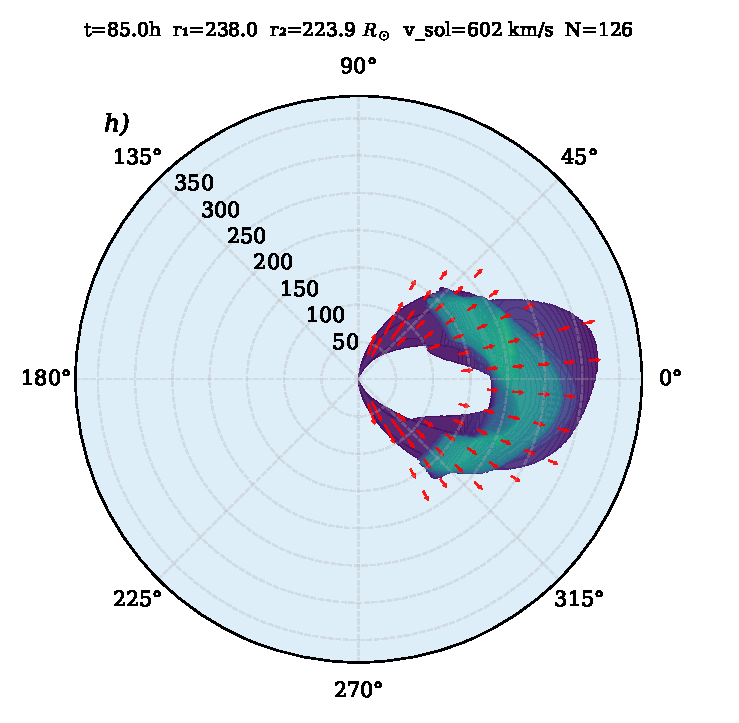
\includegraphics[width=\linewidth]{cme_conjunta_polar_panel8_s1_435_s2_1962_cropped.pdf}
        \caption*{(a)}
    \end{subfigure}
    \hfill
    \begin{subfigure}{0.555\linewidth}
        \centering
        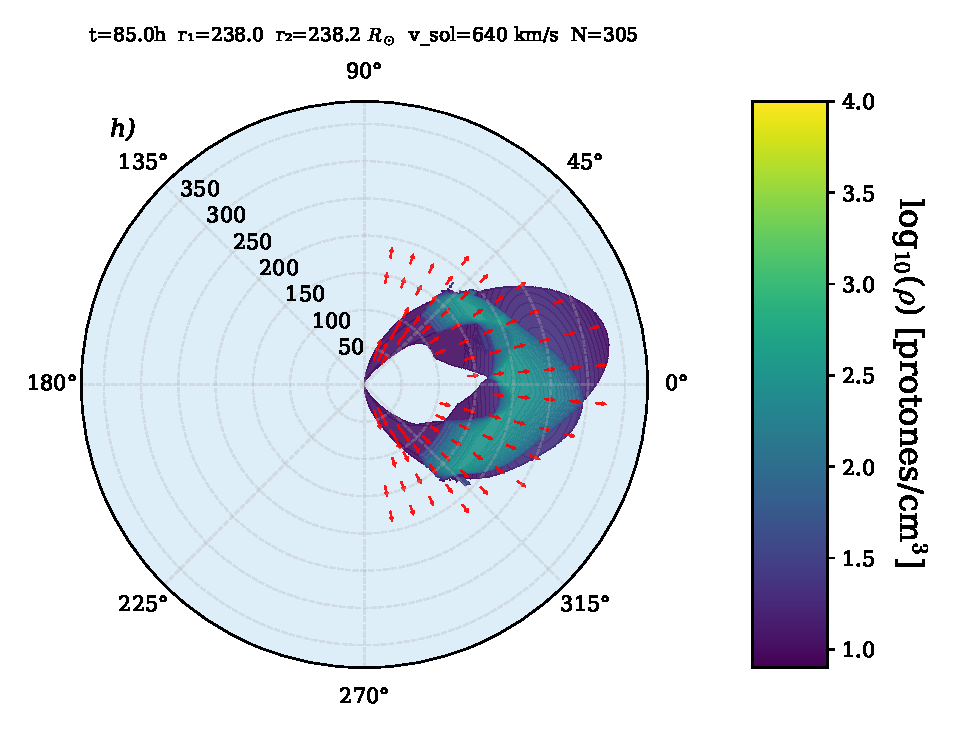
\includegraphics[width=\linewidth]{cme_conjunta_polar_panel8_s1_435_s2_256_2.pdf}
        \caption*{(b)}
    \end{subfigure}
    \caption[Comparación entre paneles finales de la simulación de la interacción de los Casos 1 y 2]{Paneles finales (85 horas) de la simulación de la evolución polar para el Caso 1 (a) y Caso 2 (b).}
    \label{fig:CMEsresultantes}
\end{figure}

Las Figuras \ref{Serietiempocaso1} y \ref{Serietiempocaso2} permiten comparar el comportamiento local de la velocidad y densidad de los casos estudiados. En el Caso 1 (Figura \ref{Serietiempocaso1}), las series temporales de densidad revelan un frente de baja densidad seguido de una región de alta densidad, ambas estructuras exhibiendo un ensanchamiento progresivo en su extensión conforme evoluciona la interacción. Asimismo, tras el paso de las CMEs, se identifica una región cuya densidad es inferior a la del medio ambiente, fenómeno atribuible al arrastre de material circundante por parte de las estructuras en interacción. La velocidad en cada serie de tiempo presenta un máximo abrupto, el cual describe un comportamiento estable de la velocidad ($\sim560$ km s$^{-1}$), seguido de un decrecimiento suave. A medida que la interacción se aleja del Sol, se observa un incremento secundario en la velocidad que se hace progresivamente más pronunciado, para luego disminuir hasta la velocidad de fondo. Este pico está asociado a una región de fusión significativa en la cual domina la velocidad de la CME precursora (CME--2), debido a la considerable diferencia entre las velocidades de ambas CMEs, puesto que la región aparece inicialmente en una zona central de la interacción y se traslada progresivamente hacia el frente de la misma, evidenciando como la CME sucesora atraviesa abruptamente a la precursora. 

Para el Caso 2 (Figura \ref{Serietiempocaso2}), la densidad en los puntos cercanos al Sol muestran dos picos, lo que indica el paso de las dos CMEs sin presentar interacción aún. Posteriormente, durante la interacción de sus extremos ($\sim 18$ horas), las densidades máximas de cada serie de tiempo describen un comportamiento decreciente para luego aumentar mientras la CME sucesora atraviesa a la precursora ($\sim30$ horas). Después este comportamiento se vuelve lineal con la distancia, puesto que el máximo de cada serie de tiempo disminuye progresivamente debido a una baja diferencia entre las velocidades de las CMEs. Asimismo, la velocidad en puntos cercanos al Sol, presenta dos valles indicando el paso de las dos CMEs con velocidades menores a la del \ac{SW}\index{Solar Wind}; en seguida los máximos de cada serie de tiempo describen el comportamiento creciente y posteriormente constante del perfil de velocidad, lo cual coincide con el comportamiento reportado por \textcite[e.g.,][]{gallagher-2003}, estabilizándose en $\sim640$ km s$^{-1}$. Asimismo, el incremento en la densidad resulta considerablemente mayor para el Caso 1 en comparación con el Caso 2 ($\sim10^3$ frente a $3\times10^{2}$ protones cm$^{-3}$), reflejando una mayor compresión asociada a una mayor diferencia de velocidad entre las CMEs. En conclusión, la interacción del Caso 2 ocurre como una fusión más suave en relación al Caso 1.
